\setchapterpreamble[u]{\margintoc}
\chapter{Caratteristiche dei materiali metallici}
\labch{cap2}

\section{Introduzione}
Le caratteristiche di un materiale dipendono dalla composizione chimica e dal trattamento termico
che hanno subito.
Le caratteristiche che citeremo sono delle caratteristiche esclusive dei materiali metallici, ma esse non sono le uniche in quanto i metalli condividono importanti proprietà con le altre famiglie di materiali. Tra le caratteristiche comuni vi è la rigidezza (anche la pietra è rigida), lo stato solido (anche il ghiaccio è solido) e la struttura cristallina, che prevede una disposizione geometrica definita degli atomi che si ripete nello spazio (ordine a lungo raggio).

Possiamo distinguere diverse proprietà che rendono i materiali metallici i più impiegati nel settore aeronautico e, in generale, in campo industriale:

\index{lucentezza}
\begin{itemize} 
    \item \textbf{Lucentezza}: in opportune condizioni i materiali metallici sono degli specchi. Questa caratteristica è stata la prima ad essere sfruttata dall’uomo: la prima applicazione dei materiali metallici è stata lo specchio in rame e la creazione di monili. Infatti, sideros, dal greco, significa oggetto che brilla. Paradossalmente, un metallo in genere non riflette la luce perché la sua superficie è ricoperta da materiale non metallico, per evitare la corrosione. Infatti, i metalli reagiscono a contatto con l’ossigeno e si ossidano, dando vita a fenomeni di ruggine. Ad esempio, l’acciaio inossidabile presenta uno strato di ossido protettivo. La lucentezza si ha quando il materiale metallico ha una superficie piana e metallica, cioè non ossidata, in quanto l’ossido non è un materiale metallico e non riflette la luce, come tutti i materiali non metallici in generale. L’ossidazione è un processo naturale e il procedimento utilizzato per rimuovere lo strato ossidato è molto costoso, quindi per riflettere si preferisce l’uso di altri materiali. La lucentezza viene, inoltre, usata per studiare la struttura dei materiali;
    \item \textbf{Conducibilità elettrica}\index{conducibilità elettrica}:i materiali metallici sono ottimi conduttori elettrici. Essi sono caratterizzati da una conducibilità di tipo ionico, tipica anche dei non metalli, e da una conducibilità di tipo elettronico, tipica dei materiali metallici. Quest’ultima è resa possibile dalla presenza del legame metallico;
    \item\textbf{Conducibilità termica}\index{conducibilità termica}: materiali metallici sono ottimi conduttori di calore grazie alla presenza di elettroni liberi di muoversi (agitazione termica), caratteristica tipica del legame metallico. Le due conducibilità sono caratteristiche molto utilizzate a livello tecnologico;
    \item \textbf{Comportamento elettrochimico}\index{comportamento elettrochimico}: i metalli si elettrizzano positivamente;
    \item \textbf{Proprietà magnetiche};
    \item \textbf{Riciclabilità}\index{riciclabilità}: non è una proprietà esclusiva dei materiali metallici (anche i vetri sono riciclabili);
    \item \textbf{Deformabilità plastica}\index{deformabilità plastica}:è la caratteristica principale dei materiali metallici. Si tratta della capacità di subire grandi cambiamenti irreversibili di forma in risposta a forze applicate e conseguente assorbimento di energia. Comporta la possibilità di produrre dei componenti meccanici sicuri, poiché non si rompono facilmente, ed è utilissima non solo nella produzione, ma soprattutto nell’impiego di tali parti. Il materiale metallico, infatti, se sollecitato fortemente si deforma prima elasticamente, come tutti i materiali, e poi anche plasticamente: ciò permette di usare tale materiale in sicurezza, poiché presenta carichi critici molto elevati, cosa che invece non accade negli altri materiali, dove si assiste a fenomeni di rottura per carichi molto inferiori. In particolare, la deformabilità può essere controllata attraverso dei meccanismi di rafforzamento, quali i trattamenti termici (trattamento superficiale). Tra le lavorazione a deformazione plastica ricordiamo la laminazione, la trafilatura e la calandratura. Dopo aver realizzato un materiale per deformazione plastica (produzione), bisogna effettuare un controllo della deformabilità, con successivi interventi di rafforzamento (trattamenti termici) e il successivo studio dei fenomeni di rottura.
    \item \textbf{Colabilità}\index{colabilità}:è l'attitudine di un materiale a riempire completamente un contenitore di qualsiasi forma una volta allo stato liquido. Le ghise hanno un’elevata colabilità e possono essere gettate in stampi con forma pressoché definitiva.

\end{itemize}

Tuttavia, bisogna trovare il giusto compromesso fra tutte queste caratteristiche. Ad esempio, se un materiale è troppo deformabile, non è abbastanza resistente. Un miglioramento si ha, ad esempio, con i meccanismi di rafforzamento, che riducono la deformabilità pratica e permettono di operare in maggiore sicurezza.

\section{Conducibilità elettrica}\label{PropElettriche} \index{conducibilità elettrica}

Tutte le sostanze che contengono ioni sono buoni conduttori di corrente, come ad esempio l'acqua. Inoltre, quando nell'acqua sono presenti altre sostanze, esse subiscono il fenomeno dell'elettrolisi e si dissociano in ioni.

I metalli sono degli ottimi conduttori; come detto nel paragrafo precedente, i materiali metallici oltre la conduzione di tipo ionico conducono anche in modo elettronico, grazie al loro caratteristico legame metallico(il quale ha il pregio di unire le caratteristiche del legame ionico a quelle del legame covalente).
Gli elettroni possiedono una certa energia e, nella struttura atomica, si posizionano in zone a loro energicamente concesse (che prendono il nome di orbitali). Queste zone sono definite come quelle in cui la probabilità di trovare l'elettrone è più alta. 
\newline \index{legame metallico}
Nel legame metallico, però, gli elettroni più esterni possono allontanarsi dal nucleo, formando u a nube elettronica mobile, detta mare di Fermi, sensibile ai campi elettrici, determinando in tal modo anche le proprietà magnetiche dei metalli.
Siccome solo gli elettroni degli orbitali più esterni hanno la possibilità di staccarsi dal nucleo, si definisce \textbf{banda di conduzione} la banda elettronica a più bassa energia tra quelle non completamente occupate.

\begin{figure}[!hbt]
	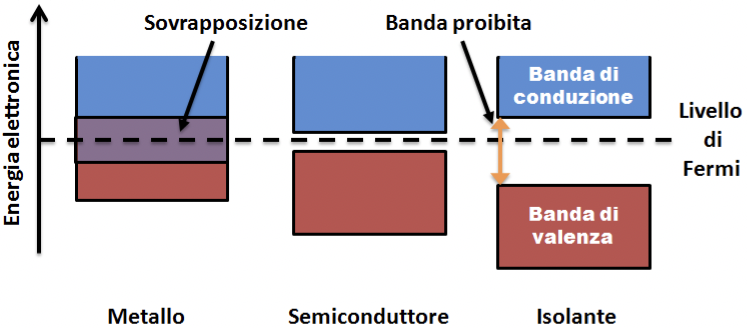
\includegraphics[width=0.6\textwidth]{images/img1.png}
	\caption[Banda di valenza]{separazione dei livelli energetici in metalli, semiconduttori e metalli}
	\labfig{img1}
\end{figure}

Tale banda, nei metalli, è parzialmente riempita e restano degli spazi vacanti \sidenote{Alla banda 's' sono legate le proprietà elettriche, alla banda 'p' quelle magnetiche}: gli elettroni che vi appartengono hanno la possibilità di spostarsi in livelli energetici diversi, divisi da un salto energetico infinitesimale, e hanno quindi un'elevata mobilità che determina l'alta conducibilità elettrica del materiale.

I metalli possono avere dei difetti reticolari puntiformi consistenti nella mancanza di un atomo nel reticolo (\textbf{vacanza} o gap) o nella presenza di un atomo estraneo (\textbf{impurità}): questi possono rappresentare dei vantaggi come degli svantaggi. Nel caso specifico della conduzione elettrica, le vacanze rappresentano degli ostacoli al passaggio di elettroni ed aumentano quindi la resistività del materiale. Il numero di vacanze è legato esponenzialmente alla temperatura: \index{vacanza}
\begin{equation*}
    \frac{\mathrm{n_{vacanze}}}{\mathrm{n_{ atomi}+n_{vacanze}}} = e^{-Q/RT}
\end{equation*}

Dove Q è il cosiddetto calore di attivazione, ovvero la quantità di energia necessaria a generare una mole di vacanze.\\

I conduttori elettrici sono fatti perlopiù di \textbf{rame}, poiché rappresentano il giusto compromesso tra conducibilità elettrica, caratteristiche meccaniche e costi\sidenote{Il rame è stato il primo metallo tecnologicamente impiegato dall'uomo (5000-6000 a.C.) perché facilmente reperibile e lavorabile. Venne poi soppiantato dal \textbf{bronzo} una lega metallica di rame e stagno, rame alluminio (bronzi all'alluminio), rame e zinco (ottoni). Solo nel 1200 a.C. si cominciò ad impiegare il \textbf{ferro}.}. \newline
Per permettere il passaggio di elettroni il metallo dev'essere il più puro possibile e con il minor numero possibile di vacanze. Il rame puro è molto costoso e difficile da realizzare. Non stupisce quindi che quello che poteva essere ottenuto nei secoli scorsi dalla fusione dei minerali era altamente impuro e quindi con una conducibilità elettrica limitata. \newline
Per ottenere rame puro si parte da quello impuro e, tramite diverse tecniche, si procede con la raffinazione.

La prima tecnica è \textbf{la fusione a zone}, che si basa sul presupposto di mettere a contatto un solido e un liquido al fine di concentrare le impurità nella fase liquida. Per comprendere questa tecnica analizziamo un diagramma di stato binario con eutettico: le curve delimitano il campo di esistenza dello stato solido e di quello liquido.
\begin{figure}[!hbt]
	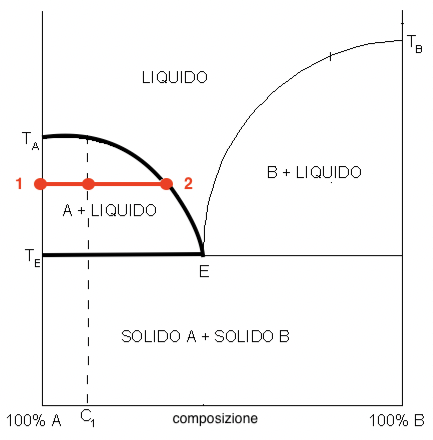
\includegraphics[width=0.6\textwidth]{images/img2.png}
	\caption[Diagramma di stato binario con eutettico]{Diagramma di stato binario con eutettico, relativo a componenti immiscibili allo stato solido e completamente miscibili allo stato liquido}
	\labfig{img2}
\end{figure}
Denotiamo con $\mathrm{T_A}$ e $\mathrm{T_B}$ le temperature di fusione di un generico solido A e B rispettivamente. Rappresentano l'origine delle curve. La curva a T costante che intercetta il punto E, detto \textbf{punto eutettico}, dove si incontrano le curve di fusione di A e B, delimita il campo di coesistenza dei due stati solidi contemporaneamente. \newline
In ascissa è riportata la composizione percentuale della miscela.\newline
Si immagini di avere un materiale solido con una percentuale $\mathrm{C_1}$ di impurità (B) e con il componente A (che supporremo sia rame) molto vicino alla purezza. Aumentando la temperatura oltre il punto di eutettico è possibile notare come la fase liquida formata contenga una concentrazione di B maggiore rispetto a quella di partenza (punto 2), mentre la fase solida resti di A puro (punto 1). Rimuovendo la fase liquida si resta, quindi, con un materiale solido puro.

La fusione può essere effettuata attraverso lo \textbf{scaldamento per induzione}: utilizzando un induttore si riscalda una porzione ristretta del materiale da cui si vogliono eliminare le impurità. In questo modo queste andranno a concentrarsi nella zona fusa del materiale e verranno trascinate dell'induttore stesso fino all'estremità del pezzo. Alla fine del processo la parte terminale dove sono concentrate tutte le impurezze viene rimossa. L'operazione può essere ripetuta più volte fino ad ottenere il livello richiesto di purezza.
\begin{marginfigure}[-5.5cm]
	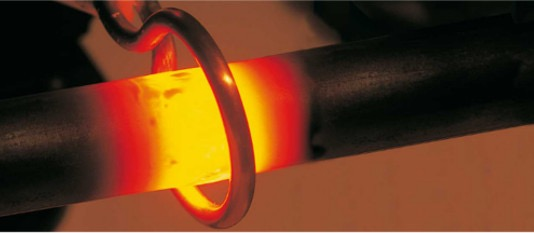
\includegraphics{images/img3.jpg}
	\caption[Fusione per induzione]{Fusione per induzione.}
	\labfig{img3}
\end{marginfigure}

Non è purtroppo possibile ottenere un materiale puro tramite questo processo: l'operazione successiva è l'\textbf{elettrolisi}. Fondendo il rame non puro ed effettuando l'elettrolisi, al catodo si depositerà il rame puro.

Questo processo di purificazione è utilizzato anche per altri materiali, quali l'\textbf{alluminio} e il \textbf{titanio}. Questi sono molto diffusi sulla crosta terrestre, ma le loro leghe sono estremamente costose da ottenere a causa delle lavorazioni necessarie per ottenerle e per renderle pure (si pensi ad esempio alle temperature necessarie per l'estrazione e l'elettrolisi), a differenza degli acciai e delle ghise che sono ottenuti con processi molto più economici. Gli acciai hanno un prezzo nell'ordine di 1€/kg, l'alluminio di 5-10€/kg e il titanio di 50-100€/kg.

Il rame puro, oltre ad avere un costo commerciale altissimo, presenta delle caratteristiche meccaniche limitate. Queste devono essere quindi migliorate con ulteriori lavorazioni o con l'introduzione di altri elementi chimici, incidendo sulle caratteristiche elettriche del materiale. \newline
Un metodo spesso impiegato in questo senso è l'\textbf{incrudimento}, un processo metallurgico in cui un materiale metallico risulta rafforzato in seguito ad una deformazione plastica a freddo (es. trafilatura o estrusione). Questo incide in primo luogo sulle caratteristiche meccaniche: aumentano limite elastico, carico di rottura e durezza, diminuiscono allungamento, strizione e resilienza. La resistività elettrica subisce un incremento e diminuisce la resistenza alla corrosione. Per questo motivo, nell'indicare in particolare tipo di rame, è necessario indicare anche il grado di incrudimento.

Il rame, sotto alcuni punti di vista, può essere considerato un inquinante, in particolare nei processi di produzione. \\
Per i materiali metallici, in particolare quelli ferrosi, esitono due tipi di processi di produzione: il primo, detto \textbf{integrale}, prevede la produzione del materiala a partire dal minerale; il secondo metodo sfrutta la \textbf{riciclabilità}, fondendo i rottami per poterne usare nuovamente il materiale. Le automobili, ad esempio, vengono costruite con materiali metallici per rispettare l'obbligo del 90-95\% di riciclabilità \sidenote{In tal senso, i materiali devono essere riciclabili non a fini energetici: spesso la riciclabilità viene utilizzata anche nell’accezione di riutilizzabilità, cioè riutilizzo del materiale stesso per produrre altri oggetti.}. I vetri e le lamiere sono riciclabili, mentre la plastica, le gomme le imbottiture dei sedili, i tessuti, etc spesso non lo sono. \\
Nel processo di rottamazione di un'automobile, l'acciaio del telaio può essere inquinato da altri composti: parti di rame, come l'impianto elettrico, e in piombo, come la batteria, possono minare la purezza dell'acciaio. Per ovviare a tale problema, durante il processo di fusione il ferro ottenuto dal rottame viene diluito con dell'acciaio "vergine" (puro) proveniente dagli scarti delle acciaierie primarie per diminuire la concentrazione dei materiali inquinanti.

Nell'ambito della conduzione elettrica, oltre al rame, vengono impiegati anche metalli preziosi come l'\textbf{oro} e il \textbf{platino}: questi, infatti, presentano una velocità di ossidazione così bassa rispetto agli altri materiali che può essere considerata trascurabile\sidenote{solo i gas nobili non si ossidano, perché non formano legami chimici}. Tale proprietà è molto utile in ambito elettronico, poiché spesso la formazione di ossidi nei circuiti può comprometterne il comportamento. Ciò può portare a conseguenze catastrofiche (si pensi a campi sensibili come il computer di bordo di un aeroplano o in campo medico o finanziario) e quindi, per evitarle, questi metalli vengono impiegati frequentemente. Il rame, per esempio, forma gli ossidi $\mathrm{Cu_2O}$ e $\mathrm{CuO}$ che non conducono corrente e danneggerebbero il dispositivo.

È evidente che non sia possibile realizzare tutti gli impianti elettrici in oro o platino, non solo per il costo proibitivo, ma anche perché presentano una resistenza meccanica bassissima, e richiederebbero quindi l'aggiunta di altri materiali, come argento o rame, o l'impiego di canaline per appoggiare i cavi.

\subsection{Trasferimento di potenza elettrica}

La potenza elettrica può essere calcolata come $\mathrm{P_{el}}=\mathrm{VI}$. \\
La potenza elettrica dissipata in un circuito di resistenza R per effetto Joule vale $\mathrm{P_{diss} = \mathrm{RI^2}}$.\\
È evidente quindi che quando si intende trasferire potenza elettrica tramite elettrodi sia necessario tenere al minimo la quantità di corrente I per limitare le perdite dissipative. Si avranno quindi, negli elettrodi, tensioni altissime (nell'ordine dei kV), con correnti tendenti a zero.\\
Dal punto di vista tecnologico, per aumentare la potenza trasmissibile, si può intervenire sulla resistenza. Per la legge di Ohm questa è pari a $\mathrm{R} = \rho\mathrm{L/S}$ dove $\rho$ è la resitività specifica del materiale, L la lunghezza del circuito e S la sia sezione.

La resistività dipende, in generale, da temperatura e composizione chimica $\rho = f(\mathrm{T, composizione})$. In particolare la resistività è funzione della temperatura poiché, con l'aumento di T, aumentano le vacanze (a causa del moto vibrazionale dei singoli atomi del reticolo\sidenote{Se viene loro fornita energia sufficiente, alcuni atomi del reticolo tendono a spostarsi verso zone superficiali (ad una maggiore energia). Questo fenomeno determina la formazione delle vacanze ed un loro movimento verso il centro del materiale, mano a mano che gli atomi interni risalgono verso la superficie.}) e, di conseguenza, la resistività e del calore dissipato per effetto Joule (questo può portare a incendi autocatalitici, ovvero in grado di alimentarsi da soli a causa di un circolo vizioso si aumento di T e $\rho$, in seguito ad un corto circuito. I salvavita servono ad impedire questa eventualità). Un modo quindi per misurare la quantità di vacanze è attraverso la misura della resistività. La temperatura porta inoltre ad un aumento del moto di agitazione molecolare, diminuendo in maniera considerevole il libero cammino medio degli elettroni, e quindi la loro capacità di trasportare corrente elettrica\sidenote{Utilizzando il cosiddetto modello di Drude (o del cammino dell'ubriaco) è possibile ricavare che $\rho \propto \mathtext{v_d}/l$ dove \mathtext{v_d} è la velocità di deriva degli elettroni, crescente con la radice di T, e $l$ è il libero cammino medio, ovvero la distanza media fra due urti successivi.}.\\
Operando su questi due parametri, in particolare sulla composizione chimica e quindi sulla scelta del materiale, si può modificare la resistenza di un circuito al passaggio della corrente e, di conseguenza, limitare la potenza persa in calore.

Si può inoltre agire sulla geometria del materiale. La lunghezza risulta spesso determinata dal problema in esame, e si opta quindi di aumentare la sezione. La soluzione sembra promettente, perché la resistenza diminuirebbe con il quadrato del diametro della sezione.\\
Comincia però a diventare preponderante il problema del peso del sistema, in particolare per sistemi in cui le potenze trasferite sono elevate come nel caso delle linee di distribuzione della corrente. Una soluzione potrebbe essere quella di ridurre il tratto libero fra due campate, avvicinando i tralicci. Nella pratica tuttavia si opta per l'utilizzo di una materiale con una bassa densità, che permetta di avere sezioni elevate con un peso contenuto. Il rame non è adatto ad applicazioni di questo tipo ($\mathrm{m/Vol} = 8930 \mathrm{kg/m^3}$), dove il materiale impiegato è invece l'alluminio: per quanto abbia una resistività specifica maggiore di quella del rame ($2,75 \times 10^{-8}\Omega\mathrm{m}$ contro $1,68\times 10^{-8}\Omega\mathrm{m}$) presenta un peso proprio molto inferiore ($\mathrm{m/Vol} = 2750 \mathrm{kg/m^3}$).

Ricapitolando, la conducibilità elettrica è affidata a:
\begin{itemize}
    \item \textbf{rame} nella maggior parte delle applicazioni elettroniche non di alta potenza;
    \item \textbf{oro o platino} nell'elettronica di precisione, dove è cruciale prevenire l'ossidazione;
    \item \textbf{alluminio} per il trasferimento di potenze elevate.
\end{itemize}

\section{Conducibilità termica} \index{conducibilità termica}

I materiali metallici conducono bene il calore grazie alla mobilità elettronica: il trasferimento di calore è infatti legato al trasporto di energia cinetica, che può essere effettuato dagli elettroni mobili. Infatti, i materiali metallici sono spesso utilizzati come conduttori termici: si pensi per esempio ai termosifoni, in cui troviamo acqua e un antigelo, e gli scambiatori di calore industriali, che possono contenere anche fluidi corrosivi. É però necessario tenere a mente che un incremento della temperatura porta spesso ad un aumento della corrodibilità del materiale.

Gli acciai vengono usati in ambiente non acido, perché il ferro si ossiderebbe e corroderebbe in seguito alla reazione seguente:
\begin{align*}
\mathrm{Fe} + \mathrm{2HCl} &\to \mathrm{FeCl_2 + H_2} \\
\mathrm{Fe} &\to \mathrm{Fe^{2+} + 2e^-} \tag{forma ionica}\\
\mathtext{2H^+ + 2e^-} &\to \mathtext{H_2} \tag{forma ionica}
\end{align*}
Il ferro non è, infatti, un metallo nobile \sidenote{La nobiltà di un metallo è determinata dalla sua capacità di resistere alla corrosione, ovvero dalla difficoltà con cui cedono elettroni. Sono considerati nobili rutenio, rodio, palladio, argento, osmio, iridio, platino, oro e alcune leghe (come l'acciaio inox).}.

Il rame si comporta in maniera differente:
\begin{align*}
    \mathrm{Cu +2HCl} &\nrightarrow \mathrm{CuCl_2 + H_2}\\
    \mathrm{Cu} &\nrightarrow \mathrm{Cu^{2+} + 2e^-} \tag{forma ionica}\\
    \mathrm{2H^+ + 2e^-} &\nrightarrow \mathrm{H_2} \tag{forma ionica}
\end{align*}

Queste reazioni non avvengono, in quanto presupporrebbero una dissoluzione anodica del rame e una reazione catodica dell'idrogeno. Ciò non avviene perché, al contrario del ferro, il rame segue l'idrogeno nella scala elettrochimica degli elementi (è più "nobile" dell'idrogeno).
Il rame viene attaccato dagli acidi ossidanti (es. acido nitrico $\mathrm{HNO_3}$).
In questi casi risultano quindi necessari materiali ceramici, come le ghise ad altissimo tenore di silicio (Si$>$10\%) o ai materiali refrattari.

Trasmettere calore significa riscaldare il materiale. Risulta quindi essenziale studiare come questo influisca sulla  formazione di un ossido, cioè sulla reazione di ossidazione. Questa reazione presenta un duplice aspetto: termodinamico e cinetico.
Dal punto di vista termodinamico, essa è sfavorita: all’aumentare della temperatura, l’ossido diventa man mano meno stabile e tende a prevalere la reazione inversa, cioè di riduzione o dissociazione dell’ossido.
Tale considerazione è, però, in contraddizione con l’esperienza: scaldando una lamiera, essa arrugginisce. Infatti, dal punto di vista cinetico, questa reazione di ossidazione è favorita dalla temperatura: aumentando la temperatura, gli ossidi si formano più velocemente, ma sono meno stabili \sidenote{Ricordiamo che i materiali metallici vengono prodotti a partire da ossidi: scaldando il materiale si riesce a separare il metallo dall'ossigeno}.

\subsection{Resistenza alla corrosione}\index{corrosione}

Prima di procedere con la conducibilità termica, analizziamo i tipi di corrosione che possono danneggiare i materiali.

Le forme di corrosione si dividono in due tipi: \textbf{corrosione elettrochimica e corrosione ossidativa}.

Il meccanismo della corrosione elettrochimica ricalca essenzialmente quello della pila, formata da un anodo (composto che cede elettroni, ovvero si ossida), un catodo (composto che acquista elettroni, ovvero si riduce) e un elettrolita.
Quando due fasi (la fase è una porzione di volume fisicamente e chimicamente omogenea) vengono a contatto, si ha la possibilità di creare una pila, detta pila di corrosione, in presenza di un elettrolita (non necessariamente liquido, basta anche l’umidità).
All’interno di un materiale possono esserci più fasi, come nell’acciaio, formato da ferro e carbonio. Una parte di carbonio si scioglie nel reticolo del ferro, dando origine a una soluzione solida omogenea, cioè uniforme in ogni suo punto e si ha un’unica fase.
La solubilità del carbonio, a temperatura ambiente, è dello 0,02\% (cella elementare CCC), ma il tenore di carbonio presente negli acciai è dell’ordine del 2\%: il carbonio dà origine a una seconda fase. Nel caso delle ghise il carbonio è presente sotto forma di grafite, mentre negli acciai il carbonio è presente sotto forma di carburi, in particolare sotto forma di cementite $\mathrm{Fe_3C}$. In un acciaio vi sono sempre due fasi: la soluzione solida di ferro e carbonio e la cementite. Vi sono, quindi, un anodo e un catodo, che possono dar vita ad una azione corrosiva di tipo elettrolitico. Questo meccanismo viene esaltato se vengono posti in contatto due metalli differenti, ad esempio l’acciaio e l’alluminio.\\
Nel passato questi metalli venivano difficilmente usati insieme per creare delle parti meccaniche. Il programma europeo Horizon 2020, impone tuttavia che le automobili debbano essere fabbricate in modo tale da produrre meno di 95g di anidride carbonica CO2 al chilometro. Dunque, per limitare le emissioni e l’inquinamento, le auto devono essere più leggere e devono necessariamente contenere molti parti in alluminio.\\
Risulta quindi importante studiare l’unione di alluminio e acciaio: il contatto tra di essi non può essere  di tipo metallico, cioè attraverso saldature o tramite bulloni e rivetti, perché la presenza di umidità porterebbe facilmente al processo corrosivo sopra descritto, coadiuvato dalle temperature generalmente elevate. Bisogna, invece, interporre un isolante, come un adesivo strutturale (resina), per giuntare due pezzi fatti di materiali metallici diversi. Il problema è che, sebbene le resine abbiano alte resistenze meccaniche e strutturali, queste crollano ad alte temperature e i pezzi non potrebbero quindi essere scaldati. Un processo critico in questo senso è quello della cottura della vernice o verniciatura \sidenote{La scocca dell'automobile prima della verniciatura viene detta BIW (Body In White) o Car Body}, che avviene circa a 185 °C.

Quindi, la corrosione di tipo elettrochimica si innesta quando due fasi diverse vengono a contatto: vi è passaggio di elettroni e scambi di energia.
La corrosione può anche avvenire in presenza di un'unica fase, quando sezioni differenti di questa sono sottoposte a condizioni ambientali o di carico differenti (corrosione da sforzo o \textit{stress corrosion}, dove la parte sotto stress si comporta in modo anodico, o corrosione per aerazione differenziale).

La corrosione ossidativa si ha quando una metallo esegue una reazione di questo tipo:
\begin{align*}
    \mathrm{Me + 1/2\, O_2 &\to \mathtext{MeO \; (ossido)}\\
    \mathtext{Me + H_2O} &\to \mathtext{Me(OH)_2 \; (idrossido)}}
\end{align*}

Il ferro si corrode per ossidazione e può dar vita a tre ossidi: $\mathrm{Fe_2O_3}$ (ematite), $\mathrm{Fe_3O_4}$ (magnetite) e FeO (wustite). Essi si formano in base alle condizioni al contorno: hanno massa volumica differente tra loro e differente dal metallo base, e danno quindi origine ad uno strato poroso, estremamente friabile e non uniforme, che non è sigillante per il metallo base. La ruggine, infatti, non isola e non protegge il metallo base dall’ambiente esterno, permettendo agli altri agenti corrosivi di entrare in contatto con il metallo base. In altre parole, uno strato di ossido non è una superficie \textbf{passivante}, cioè non è chimicamente inerte di fronte all’azione degli altri agenti corrosivi.

Gli ossidi dell’alluminio, che genera l’ allumina $\mathrm{Al_2O_3}$, e del titanio, il cui ossido prende il nome di rutilo $\mathrm{TiO_2}$, hanno un comportamento analogo fra loro, ma assolutamente differente rispetto a quello del ferro. Infatti, sia l’allumina sia il rutilo sono perfettamente aderenti e sigillanti nei confronti della superficie del metallo di base e dunque protettivi: la superficie del metallo sottostante rimane isolata dall’ambiente esterno e viene bloccata qualsiasi azione corrosiva esterna. Si dice che l’alluminio e il titanio sono \textbf{autopassivanti}\index{autopassivazione}. Gli strati sono sottilissimi (pochi piani atomici) e compatti e hanno un grande potere protettivo. Questi due metalli risultano quindi formalmente inossidabili, nel senso che non vengono corrosi in profondità dalla presenza dell'ossigeno\sidenote{I cosiddetti allumini anodizzati sono lavorati elettrochimicamente per aumentare lo spessore dello strato ossidato. Al contrario però di quello che si potrebbe pensare, questo processo non rende il metallo più resistente all'attacco dell'ossigeno. Se, infatti, un graffio esponesse parte del metallo base questo ossiderebbe subito, sigillando nuovamente il materiale. Il processo è quindi sostanzialmente una misura estetica.}.

Nel caso degli acciai, non si può ha l’autopassivazione a causa della formazione degli ossidi di ferro. \index{acciai inossidabili}
Tuttavia, si può ottenere un comportamento simile a quello dell’alluminio e del titanio  se è presente un terzo elemento come il cromo Cr, in percentuali almeno maggiori al 13\%.\\
Il cromo è spesso presente in molti acciai perché è un materiale economico, ma la sua quantità varia fra il 3 e il 4\%: in questo caso, lo scopo della sua presenza è l’agevolazione del processo di tempra.
Per avere un acciaio inossidabile, il cromo deve dunque essere presente in tenori maggiori del 13\% perché in queste condizioni si forma uno \textbf{spinello}, cioè un ossido formato da una parte bivalente e una parte trivalente: $\mathrm{FeO\cdot(Fe,Cr)_2O_3}$.
Questo composto sostituisce completamente gli ossidi del ferro e si comporta come allumina o rutilo, rendendo la superficie autopassivante, dando vita agli \textbf{acciai inossidabili} (INOX o stainless steel).

Se vogliamo che l’acciaio resista sia alla corrosione sia elettrochimica che corrosiva, esso deve, di norma, essere \textbf{monofasico} \sidenote{Da un punto di vista microstrutturale, nei materiali monofasici la fase costituente può essere formata da
un unico dominio, dotato di continuità ed esteso all’intera dimensione del manufatto o da insiemi di più domini distinti e contigui, di dimensioni finite (grani o cristalliti).}. É possibile classificare gli acciai in base alla fase prevalente della struttura.\\
Si parla di acciai 18-8 o AISI 304 se, oltre a ferro e carbonio\sidenote{come vedremo, quest'ultimo nel minor tenore possibile per evitare la formazione di carburi}, sono presenti 18\%  di cromo e l’8\% di Nichel. La presenza di quest’ultimo è necessaria per poter estendere il campo austenitico fino quasi a temperatura ambiente (questa resta presente come fase metastabile, ma la sua trasformazione in perlite a temperatura ambiente richiederebbe tempi biblici), e l'8\% è il tenore di Nichel minimo per avere tali strutture con la presenza di cromo, che è un elemento ferritizzante\sidenote{che favoriscono la formazione delle ferriti $\alpha$ o $\delta$}. Gli acciai di questo tipo si dicono quindi \textbf{acciai austenitici}\index{acciai austenitici}, con formazione dello spinello $\mathrm{(Fe,Ni)O\cdot(Fe,Cr)_2O_3}$: sono i più costosi, poiché sebbene il ferro e il cromo siano abbastanza diffusi sulla crosta terrestre, il nichel è concentrato solo il alcune zone della terra ed molto difficile da produrre\sidenote{Germania e Italia, durante la Seconda Guerra Mondiale, a causa di embraghi vari ed eventuali, non avevano accesso a giacimenti di nichel. Dovendosi adattare siamo diventati grandi esperti di acciai INOX, anche se il meglio che siamo riusciti a cacciare, un acciaio a Mn-N, era comunque scarso rispetto a quelli belli belli in nichel. Per quanto non abbiano le migliori caratteristiche meccaniche, l'assenza del nichel, che è un allergene, rende attrattivi questi acciai in ambito medico.}. Presentano ottime caratteristiche meccaniche, sono facilmente lavorabili e saldabili e non presentano caratteristiche magnetiche a causa della presenza della struttura CFC. Non per l'assenza di un punto critico di cambiamento di fase non possono essere temprati.
In realtà, oggigiorno tale acciaio è stato soppiantato per questioni legali: si producevano acciai con tenori di Nichel del 7,5\% per risparmiare e non vi era la presenza monofasica di ferro CFC, bensì anche la presenza di ferro CCC, cioè di ferrite. Si utilizza il 20-10, per assicurare una struttura completamente austenitica e quindi monofase.

 Il tallone d’Achille degli acciai autentici è la non resistenza alla stress corrosion e al pitting, che causa tensioni meccaniche.
 
Comportamenti analoghi sono raggiungibili dagli acciai \textbf{ferritici}\index{acciai ferritici}, in cui non vi è il nichel e il cromo è presente con tenori superiori al 15\%: ciò rende questa famiglia di acciai meno costosi di quelli austenitici. La presenza di carbonio, austenitizzante, porta il tenore di Cr richiesto per la completa eliminazione della fase $\gamma$ intorno al 17 $\div$ 20\%.
Essi, però, non possono essere utilizzati a basse temperature perché rompono fragilmente, in quanto hanno una temperatura di transizione duttile-fragile poco inferiore rispetto a quella ambiente\sidenote{Questo problema affligge in genere tutti gli acciai con struttura CCC. Per qualche esempio spettacolare si cerchi "navi Liberty, Seconda Guerra Mondiale"}. Reagiscono molto meglio degli austenitici alla stress corrosion. Hanno delle buone caratteristiche meccaniche, che però non possono essere incrementate mediante trattamenti termici a causa dell'assenza della fase austenitica. Hanno una bassa saldabilità.\\
Sono utilizzati nella produzione di lavelli.

In questa tipologia di acciai, sia ferritici che austenitici, il tenore di carbonio deve essere il più basso possibile, anzi preferibilmente nullo, in quanto la sua presenza genera la seguente reazione: $\mathrm{Cr + C \to Cr_xC_y}$, cioè origina carburi di cromo, che sono doppiamente nocivi per il materiale perché da un lato formano una seconda fase, dall’altro causano una depauperazione di cromo, dove si formano i carburi, rendendo l’acciaio molto meno resistente alla corrosione e causando una corrosione intergranulare. Gli acciai con bassissimo tenore di carbonio sono indicati con la lettera "L" dopo la sigla.

Dato che il processo di eliminazione del carbonio è molto costoso, esso viene neutralizzato e reso meno nocivo con l’introduzione di titanio niobio o di vanadio: questi tre elementi hanno un’affinità elettronica col carbonio maggiore di quella del cromo, e dunque si formeranno i carburi di titanio o di vanadio, dando vita ai cosiddetti \textbf{acciai stabilizzati}\index{acciai stabilizzati} al titanio-niobio- vanadio. Se da un lato vi è lo svantaggio di aggiungere una seconda fase, dall’altro, si ha però una matrice inalterata in termini di tenore di cromo, e dunque resistente alla corrosione con resistenze di 200-300 MPa (marmitte).
Per migliorarne le caratteristiche meccaniche senza aggiungere altri elementi, si usa l’incrudimento, che però peggiora la resistenza a corrosione, in particolare alla stress corrosion.

Per unire le qualità di queste due famiglie sono stati creati degli acciai duplex, cioè acciai bifasici \textbf{austeno-ferritici}. Essendo presenti due fasi, si sacrifica un po’ di resistenza a corrosione per guadagnare di resistenza alla stress corrosion. Si usano soprattutto per l’impiantistica.
Infine, esistono anche gli acciai \textbf{martensitici}\index{acciai martensitici}. La martensite è una fase metastabile formata da ferro e carbonio: mentre la ferrite e l’austenite sono fasi presenti nel diagramma di stato in condizioni di equilibrio, la martensite non è presente poiché non è una fase di equilibrio. Essa si ottiene violentando di fatto il sistema, ad esempio raffreddando velocemente a partire da alte temperature, non dando al carbonio il tempo necessario per diffondere e dare vita alla cementite.
La martensite è una soluzione sovrasatura di carbonio, cioè è presente una quantità di carbonio superiore al valore termodinamicamente concesso ed ha un reticolo molto tensionato. In queste condizioni, la struttura cubica si deforma in una struttura tetragonale molto allungata, che contiene circa lo 0,2\% di carbonio (serve a deformare la ferrite e dara durezza) e dal 15 al 20\% di cromo (serve per l’inossidabilità e la creazione dello spinello), mentre il nichel è totalmente assente. Sono in genere molto duri perché la struttura martensitica è molto tensionata e sono gli unici acciai inossidabili che possono essere temprati.\\
Sono acciai molto usati, ad esempio, nei coltelli, in quanto non devono essere soggetti all’azione della ruggine e possedere una certa durezza per no perdere il filo. 

È, ovviamente, possibile proteggere i materiali metallici dalla corrosione anche senza fare uso di leghe inossidabili.\\
Il primo metodo, e il più semplice ed economico, è la verniciatura. Questa soluzione non è particolarmente resistente poiché ogni graffio sulla vernice che esponga il metallo sottostante ne compromette l'efficacia. È possibile apportare uno strato di materiale più resistente, come ad esempio di piombo (lamiere piombate).\\
Un metodo efficace si basa sull'utilizzo di una patina di zinco: questo metallo, essendo più anodico del ferro, si carica del fardello dell'ossidazione, risparmiandone l'acciaio sottostante con indomito coraggio e spirito di abnegazione\sidenote{Grazie eroe}. La deposizione dello zinco avviene principalmente in tre modi:
\begin{enumerate}
    \item Galvanizing: la lamiera da trattare viene immersa in un bagno di Zn e Al al fine di incoraggiare la diffusione dello zinco nel reticolo del ferro e viceversa. Lo spessore viene poi controllato mediante due getti d'aria. L'aggancio è indiscutibilmente molto buono.
    \item Elettrodeposizione: lo Zn viene depositato tramite il medesimo processo elettrochimico che avviene nelle pile. Gli strati che si possono ottene sono nell'ordine dei $\mu$m, decisamente troppo sottili per poter essere considerati sicuri (il problema sarebbe lo stesso della vernice). Si usa passivare lo strato di Zn tramite dei materiali protettivi. Fino a qualche anno fa si usava la passivazione al Cr, molto bellina perché dava un colore dorato alla  lamina. Il fatto che il Cr sia stato annoverato nel club dei materiali cancerogeni ne ha fatto tramontare la brillante carriera, ed è oggi sostituito principalmente da silani.
    \item Vernici prezincate: sono vernici con un altissimo contenuto di Zn. Queste vernici offrono un appiglio ottimo per le verniciature successive, e sono quindi molto utilizzate.
\end{enumerate}
Invece di proteggere il Fe con un metallo più anodico è possibile renderlo catodico rispetto all'ambiente tramite un apporto di energia elettrica. Il metodo funziona, ma è molto dispendioso in termini di energia.

La prova principe per la valutazione della resistenza alla corrosione è la cosiddetta nebbia salina: il pezzo viene lasciato per 500h in un atmosfera con un contenuto controllato di NaCl o altri sali e viene registrato il tempo necessario alla formazione di ossidi. Spesso vengono praticate incisioni (scratches) per rendere più evidente il processo.

%Spostare questa sottosezione dopo l'altro tipo di corrosione
\subsubsection{Il problema dell'idrogeno}\label{problema idrogeno}
Nel campo dei fenomeni elettrochimici, in presenza di acqua, oltre all’azione corrosiva, si ha anche sviluppo di idrogeno:
\begin{equation*}
    \mathrm{Fe + 2H^+} \to \mathrm{Fe^{2+} + H_2}
\end{equation*}
Infatti, una soluzione acquosa comporta lo sviluppo d’idrogeno in una reazione elettrochimica.\\
Essendo l’idrogeno un elemento piccolo, esso può penetrare facilmente nei materiali, sotto forma atomica: esso può essere rimosso attraverso la deidrogenazione. Se ciò non avviene, esso si posiziona nei bordi di grano, nelle vacanze o nelle dislocazioni, che sono difetti superficiali, puntuali e lineari dei metalli, ovvero nelle cosiddette "trappole". Qui l’idrogeno atomico assume la forma molecolare biatomica: $\mathrm{2H} \to \mathrm{H_2}$. A tale reazione è associato, però, un aumento di volume che causa il tensionamento del materiale fino al punto di rottura. Quindi, oltre alla corrosione, vi è anche l’infragilimento del materiale.\\
La deidrogenazione deve essere effettuata prima che l’idrogeno entri nelle trappole, cioè al massimo una o due ore dal momento del rilevamento della presenza di idrogeno.
Il materiale viene riscaldato fra i 180 °C e i 200 °C, per gli ingranaggi piccoli e gli acciai, per un tempo che va dalle 4 - 5 ore alle 48 ore, per i pezzi di uso aeronautico. Infatti, scaldando il materiale, l’idrogeno va via. Ovviamente, la temperatura e il tempo variano con le dimensioni del pezzo: un grande lingotto necessità di una temperatura di 600 °C e circa una settimana di tempo.\\
L’idrogeno può penetrare in un materiale anche quando si hanno processi di \textbf{elettrodeposizione} o processi galvanici, come zincatura, cromatura, nichelatura, cadmiatura, etc, attraverso i quali si deposita un materiale su un componente e durante i quali l’idrogeno si scarica al catodo, o nei processi di deformazione a caldo o a freddo, con l’utilizzo di acido solforico o cloridrico per l’eliminazione dello strato di ruggine o di ossido.\\
Lo sviluppo di idrogeno può anche avvenire quando si ha un pezzo incandescente in presenza di vapore acqueo: ad alte temperature (come accade nelle saldature o nei trattamenti termici) avviene il cracking (rottura) della molecola d’acqua, che comporta lo sviluppo di idrogeno, che entra nel materiale:
\begin{align*}
    \mathrm{CH_4 + O_2} &\to \mathrm{CO_2 +H_2O}\\
    \mathrm{CH_4 + O_2} &\to \mathrm{CO_2 +H_2} \tag{in rarefazione di ossigeno}\\
    \mathrm{2CO} &\to \mathrm{C + CO_2}
\end{align*}
Le atmosfere tipicamente ottenute nella combustione sono CO, $\mathrm{CO_2}$, $\mathrm{H_2}$, $\mathrm{H_2O}$, $\mathrm{N_2}$.

L’idrogeno è molto pericoloso perché è subdolo, come il monossido di carbonio: è difficile verificare se esso è penetrato nel materiale, in quanto non altera le proprietà meccaniche del materiale immediatamente. A un certo punto, però, si può verificare una \textbf{frattura differita}, chiamata così perché il fenomeno di danneggiamento avviene anche molto tempo dopo rispetto a quando l’idrogeno è entrato nel materiale (anche settimane o mesi). L’idrogeno, infatti, penetrando nelle microcricche e gonfiandosi, può creare l’avanzamento di quest’ultime. Quando ciò avviene, il materiale si rompe con carichi di gran lunga inferiori al carico di snervamento e si spacca in modo fragile, senza cioè nessun preavviso, a causa delle tensioni generate dall'aumento di volume dell'idrogeno.\\
Le fratture differite, che sono il pericolo più grande in cui si incorre con la presenza di idrogeno, si hanno solo per materiali con resistenze maggiori a 900 MPa, limite sotto il quale l’idrogeno non genera pericoli. Infatti un materiale poco resistente può deformarsi per accomodare l'espansione dell'idrogeno, ma se il materiale non si deforma, quindi è molto resistente, le tensioni dovute all’aumento di volume dell’idrogeno portano ad una rottura fragile del materiale. Questo problema è diventato rilevante solo recentemente: per alleggerire le autovetture si impiegano oggigiorno acciai che superano anche a 1500 MPa di resistenza, e che quindi potrebbe rompersi per idrogenazione. Prima, per la carrozzeria si usavano acciai con resistenze intorno ai 200-300 MPa. E’ diventato importante, quindi, valutare la resistenza dei materiali dopo l’introduzione dell’idrogeno.
Un altro fattore da considerare è la struttura del materiale ed in particolare il volume degli interstizi.
Il ferro, ad esempio, presenta due configurazioni allotropiche differenti:
\begin{itemize}
\item \textbf{Ferro cubico a corpo centrato CCC} (ferrite): presenta 8 atomi ai vertici e un atomo al centro;
    \item \textbf{Ferro cubico a facce centrate CFC} (austenite): presenta 8 atomi ai vertici e 6 atomi al centro (uno per faccia).
\end{itemize}
\begin{figure}[!hbt]
	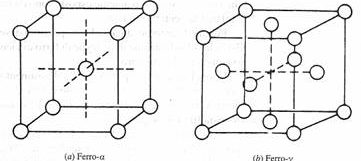
\includegraphics[width=0.6\textwidth]{images/img4.png}
	\caption[Configurazioni allotropiche ferro]{Configurazioni allotropiche del ferro: a sinistra la struttura CCC, a destra la CFC}
	\labfig{img4}
\end{figure}
Nella configurazione CFC lo spazio libero è 5 volte maggiore di quello nella CCC: questo permette all'idrogeno di essere assorbito all'interno delle cella, e lascia maggiore spazio a disposizione per l'espansione dell'idrogeno molecolare \sidenote{Ciò si collega alla solubilità del carbonio nel ferro: nella configurazione CFC, essa è del 2\%, contro lo 0,02\% della configurazione CCC.}.
 La transizione da CCC a CFC avviene a circa 700°C. Le conseguenti variazioni di volume, che non avvengono in maniera omogenea possono creare tensionamenti e conseguenti rotture. Infatti, quando viene sottoposto a trattamenti termici, il cuore del materiale si riscalda (o raffredda) più tardi rispetto alla superficie; inoltre, quando il cuore di espande (o contrae), nel materiale si genera uno stato tensione di trazione (o di compressione) che causano la rottura del materiale.
 
 Nella configurazione CCC, gli interstizi sono molto più piccoli rispetto alla configurazioni CFC: essa è molto più critica e più soggetta a rottura per idrogeno.
La peggiore soluzione di tutte sarebbe scegliere un materiale con celle in configurazione CCC e con resistenza superiore ai 900 MPa: sicuramente, i danni dovuti all’ingresso di idrogeno sarebbero gravissimi.\\
Le leghe di alluminio e zinco 7000 sono molto usate in aeronautica, ma non in campo automobilistico. Le leghe di serie 7000 presentano resistenze intorno ai 600-700 MPa e configurazioni di tipo CFC, però presentano dei precipitati intermetallici, le cui conseguenze non sono note.
E’ fondamentale, quindi, studiare il materiale nelle sue peggiori condizioni, cioè materiale non vergine dopo che ha subito una deformazione. Se vi è la presenza di idrogeno, bisogna stabilire i carichi che portano a rottura il materiale e verificare cosa accade per carichi pari al 5-10\% del carico di snervamento (molto utile in campo automobilistico). Si deve, inoltre, considerare la possibilità dell’elettrolisi dell’acqua, in cui il materiale funge da catodo, e verificare cosa accade in condizione di saturazione dell’idrogeno.

La suscettività o risposta di un materiale alla presenza di idrogeno può essere valutata con
metodi diversi:
\begin{itemize}
    \item si può appendere il materiale, metterlo in trazione e posizionare un carico al di sotto di esso:
inserendo man mano idrogeno, si può studiare la sua reazione;
\item si può usare il metodo U-band, che prevede di piegare una lamiera a forma di U, imbullonarla
e usarla come catodo immergendola in una soluzione, dove si ha la scarica di idrogeno;
\item l’ultimo metodo prevede l’uso di un anello con due fessure: il materiale viene inserito e
trazionato fino ad una certa deformazione $\varepsilon$ ed una certa tensione $\sigma$. Successivamente viene imbullonato a delle piastre e tolto dalla macchina, per mantenere lo stato di tensione, ed immerso in un fluido elettrolita, per studiarne il comportamento. L’acqua si scaricherà all’anodo, il metallo al catodo: 
\begin{align*}
    \mathrm{2H^+ + 2e^-}&\to \mathrm{2H}\\
    \mathrm{4OH^-}&\to \mathrm{2H_2O + O_2}
\end{align*}
\end{itemize}

\subsubsection{Radiatori} \index{radiatori}

I radiatori per uso civile (termosifoni) possono essere fatti con tre diversi materiali:
\begin{itemize}
    \item ghisa
    \item alluminio
    \item acciaio
\end{itemize}
Potrebbero anche essere fatti in rame ma non vengono costruiti per ragioni di costo: il rame viene utilizzato solo in ambito industriale.\\
Questi materiali però non sono fra loro intercambiabili, ma ognuno di essi ha una collocazione ben specifica.\\
I radiatori in ghisa si trovano in costruzioni antiche per avere una cessione progressiva del calore, i radiatori in alluminio si trovano nelle costruzioni recenti per avere una cessione immediata del calore, mentre l’acciaio viene utilizzato al posto dell’alluminio per ragioni di costo.\\
In passato, circa 40 anni fa, le case erano abitate 24 ore al giorno, quindi era necessario un riscaldamento progressivo, per garantire il calore per tutta la giornata. Serviva un materiale dotato di una notevole inerzia termica, quindi una grande capacità di accumulare calore, e che potesse rilasciare il calore gradualmente: si utilizzava la ghisa.\\
Oggigiorno, invece, interessa avere rapidamente del calore e per brevi periodi di tempo, quindi una fornitura di calore concentrata in un tempo ridotto. Serve un materiale che abbia un elevato coefficiente di conduzione termica (o scambio termico) come l’alluminio. Infatti, le nuove case devono riscaldarsi in un lasso di tempo ridotto.\\
Si distinguono diverse modalità di riscaldamento (metallurgia politica).\\
Un tempo si utilizzavano le stufe a carbone, camini e bracieri; solo in epoca relativamente recente si è passati al riscaldamento centralizzato.\\
Dopo la crisi energica del 1972, però, si è passati al riscaldamento autonomo (individuale), dove ogni alloggio è dotato di una propria caldaia.\\
Con questa soluzione, il dispendio di energia è risultato più di quanto si pensasse, e dunque al giorno d’oggi, se vi sono almeno quattro unità immobiliari, è previsto un impianto centralizzato. Tale tipo di impianto conviene per coloro che vivono la casa e necessitano di un riscaldamento prolungato nel tempo, mentre quello autonomo viene acceso solo quando vi è bisogno.\\
Si è tornati al riscaldamento centralizzato per controllare i consumi e l’inquinamento ambientale, che viene ridotto e controllato. Infatti, dal 31/12/2016 sarà obbligatorio l’uso di un’unica caldaia super efficiente. Questa è la motivazione ufficiale. In realtà\sidenote{Scavino feat. Qanon\index{Qanon}}, se vi sono caldaie singole, quindi con il riscaldamento autonomo, ogni locatore fa un proprio contratto con l’ente fornitore e in caso di morosità, l’ente deve comunque fornire il gas perché possono esserci cause di forza maggiore che impediscono il pagamento e il gas non può essere limitato. Nel caso di riscaldamento centralizzato, se un locatario non paga, pagano gli altri condomini. Quindi, alla base di tale decisione vi è un motivo economico e legale.

Il discorso è diverso per l’erogazione dell’elettricità: i contatori vengono cambiati per facilitarne la lettura e gli interventi tecnici. La corrente elettrica può essere limitata, a differenza del gas, se vi è morosità, poiché esiste una soglia minima stabilita. Quindi, vi è la possibilità di limitare la singola utenza.

\section{Saldatura}\index{saldatura} %guarda pagina wikipedia inglese

Le proprietà termiche ed elettriche dei materiali metallici confluiscono nella saldabilità.\\
La saldatura è una tecnica di giunzione dei materiali metallici mediante la quale si crea un continuo; essa prevede di arrivare alla fusione delle parti da giuntare e la successiva cosolidificazione.

La saldatura può avvenire anche con l’uso di un metallo di apporto: due pezzi di materiali metallici
(sia differenti sia non) possono essere saldati introducendo fra essi un metallo di apporto, che unisce i due pezzi cosolidificandosi con loro. Viene chiamato anche cordone di saldatura e deve essere un metallo più nobile dei primi due perché, essendo una parte localizzata, l’azione corrosiva deve interessare i componenti e non il metallo d’apporto, che non deve corrodersi.

Si parla di \textbf{brasatura}\index{brasatura} quando arriva a fusione solo il metallo d’apporto e non gli altri due materiali metallici. In questo caso, il metallo d’apporto è più bassofondente rispetto ai due metalli che si devono giuntare: ne sono un esempio le leghe di stagno, di zinco, di argento che devono essere saldate con il rame, che fonde ad una temperatura di circa 1300 °C.

Un caso intermedio è la saldobrasatura, una tecnica di giunzione che prevede la fusione solo di uno dei due materiali: ne sono un esempio le leghe di alluminio, che fondono a circa 550 °C, saldate con le leghe di ferro, cioè acciaio, che fondono a circa 1300-1400 °C. La temperatura di fusione dell’alluminio è di 654°C, quella dell’acciaio 1537°C, quindi è logico che sia il solo alluminio a fondere. Viene usata in giunzioni fra materiali con caratteristiche molto diverse.

Le tecniche di saldatura sono molte, e analizzarle sarebbe molto complesso.\\
Una tecnica molto rudimentale è quella operata tramite il cannello ossiacetilenico, mentre tecniche più sofisticate sono l’utilizzo dell’arco elettrico: quando si porta un’elettrodo ad una distanza opportuna dal pezzo, entrambi immersi in un aeriforme (gas o vapore), scocca l'arco elettrico, che fonde il materiale metallico dell'elettrodo, il rivestimento ed il metallo del pezzo che deve essere saldato. Tra i vari sistemi di saldatura ad arco elettrico a filo continuo, ricordiamo la saldatura MIG (Metal-arc Inert Gas) o MAG (Metal-arc Active Gas), in cui l’unica differenza è nel gas che viene usato per la protezione del bagno di saldatura, di solito una miscela di di Argon e CO2 oppure solo CO2. Esiste, poi, anche la saldatura ad elettrodo o TIG (Tungsten Inert Gas), un procedimento di saldatura ad arco con elettrodo infusibile, cioè non consumabile, di tungsteno, sotto protezione di gas inerte, che può essere eseguito con o senza metallo di apporto e non prevede il contatto della saldatrice con i pezzi da saldare. In tutti i casi, l’ambiente deve essere neutro per proteggere la zona di saldatura dagli inquinanti.

Un altro metodo molto utilizzato è quello dello spot welding (saldatura a punti), soprattuto in campo automobilistico, che si basa sulla generazione di calore per effetto Joule. Poste le lamiere da saldare fra due elettrodi (solitamente in rame), vi viene fatta scorrere della corrente. Il punto di contatto fra le lamiere, poiché viene interrotta la continuità del materiale, è il punto con la più alta resistività e quindi anche il punto che si scalderà maggiormente. Come nel caso del corto circuito analizzato nella sezione \ref{PropElettriche}, l'incremento di resistività con la temperatura fa si che questo fenomeno si autoalimenti, portando alla fusione nel punto di contatto, detto nocciolo.
L'alluminio presenta dei problemi con questo tipo di saldatura, perché tende, con l'aiuto della corrente elettrica, a corrodere gli elettrodi di rame.
\begin{marginfigure}
        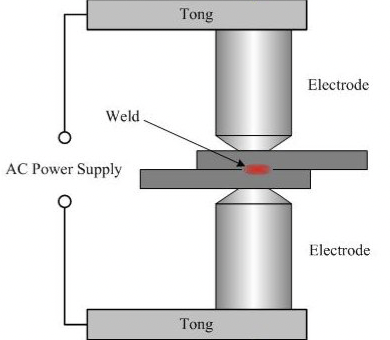
\includegraphics{images/img5.png}
        \caption[Spot Welding]{Spot welding}
        \labfig{img5}
\end{marginfigure}

La domanda che ci poniamo ora è: \textit{quale tra acciaio ed alluminio è
il materiale più facile da saldare?}\\
Da un lato la temperatura di fusione dell’alluminio (654 °C) è molto
minore di quella del ferro (1537 °C), dall’altro per la legge Delong-
Petit sappiamo che si arriva a fusione quando si fornisce un’energia
sufficiente a distruggere tutti i legami interatomici, raggiungendo una determinata temperatura. Quindi dobbiamo concentrare la nostra attenzione sull’energia necessaria per arrivare a fusione: sia l’alluminio sia il ferro sono caratterizzati dal legame metallico, quindi l’energia necessaria per rompere i legami è spannometricamente la stessa.\\
Quindi, la differenza di temperatura di fusione si può spiegare con il fatto che la capacità termica dell’alluminio (cioè il calore da fornire per aumentare la temperatura) è molto maggiore di quella del ferro. Assorbendo molta più energia di quello che serve per scaldarsi e aumentare di temperatura, l’alluminio fonderà a una temperatura minore di quella del ferro, perché ha già assorbito tanta energia, che non riesce più a trattenere. L’alluminio, infatti, ha una conducibilità termica molto elevata: sebbene richieda molta energia, esso non è capace di mantenerla e la dissipa.\\
Se si opera tramite spot welding, cioè saldatura a punto o a resistenza, la situazione peggiora perché l’alluminio ha anche una minore resistività del ferro, cioè una minore resistenza elettrica e quindi una maggiore conducibilità elettrica: ciò rende questo materiale molto più ostico da saldare rispetto al ferro. Tuttavia, per aumentare la resistenza elettrica si può inserire un foglio di zinco o si può aumentare lo strato di ossido, che non e conduttivo e genera resistenza.\\
Quindi, per fondere l’alluminio vi è la necessità di saldatrici più potenti rispetto a quelle usate per il ferro, anche se la temperatura di fusione di quest’ultimo è molto più elevata: la saldatura dell’alluminio è, quindi, onerosa e difficile.   \\
Spesso, inoltre, non è possibile saldare le leghe di alluminio, in quanto sono leghe ad elevate prestazioni meccaniche (duralluminio Al+Cu, Al+Zn, Al+Li), perché la resistenza meccanica crollare si superano i 100/150 °C. Tecnologicamente, non conviene saldare tali leghe.

Infatti, la saldatura è un trattamento termico che può modificare le caratteristiche del materiale metallico. Analizziamo il processo nello specifico: il materiale viene portato a fusione nella zona di fusione (fusion zone), mentre nelle zone limitrofe non si arriva a fusione, ma sono comunque fortemente riscaldate. Esse vengono chiamate ZTA, cioè Zone Termicamente Alterata (in inglese HAZ, Heat-Affected Zone), e sono il vero punto critico delle saldature. Accanto alle ZTA abbiamo il cuore inalterato del materiale (in inglese bulk), che
subisce un lieve riscaldamento o del tutto nullo. Se la saldatura non è fatta bene e il pezzo si rompe in corso d’opera, esso si rompe nel cordone di saldatura: questo tipo di rottura può essere dovuto ad una superficie sporca, alla presenza di grandi cavità o porosità interne.
\begin{figure}[hb]
    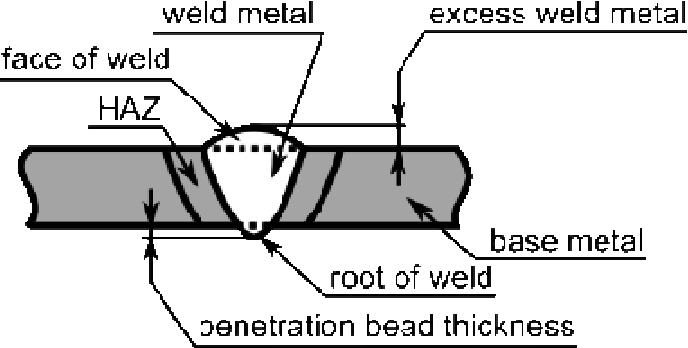
\includegraphics[width=0.6\textwidth]{images/img6.png}
    \caption[Schema saldatura]{Schema di una saldatura}
    \labfig{weldingscheme}
\end{figure}

Se la saldatura è fatta bene e il componente si rompe in corso d’opera, esso si rompe nella ZTA. Esse sono le zone critiche perché riscaldandosi tendono a dilatarsi, ma avendo il cuore freddo inalterato a fianco che fornisce un’elevata resistenza a questo movimento, le ZTA vanno in compressione e il cuore in trazione. Nasceranno dunque delle tensioni interne, che aumenteranno nella fase di raffreddamento. Infatti, in questa fase, le ZTA cercano a contrarsi perché si raffreddano prima, ma il cuore caldo impedisce tale movimento. Di conseguenza, le ZTA vanno in trazione e il cuore in compressione.\\
Inoltre, a basse temperature, il materiale è poco deformabile e se le azioni di trazione sono notevoli, il pezzo può andare incontro a rottura proprio nella ZTA, perché i materiali metallici sopportano molto male le sollecitazioni a trazione. Una modo per evitare rotture improvvise può essere quella di raffreddare più lentamente possibile. L’acqua è il mezzo peggiore per raffreddare i materiali metallici.

Queste considerazioni non riguardano solo le saldature, ma in generale tutti i trattamenti termici, che comportano un riscaldamento e un conseguente raffreddamento di velocità variabile: se il raffreddamento è lento si ha la ricottura, se è più veloce si ha la tempra.\\
Un particolare tipo di raffreddamento si ha in aria calma, con un procedimento chiamato normalizzazione, che sarà più simile alla ricottura per un pezzo di grandi dimensioni, più simile alla tempra per i pezzi più piccoli.

I pezzi da saldare non sono punti isolati nello spazio, bensì sono reali essi hanno una superficie, un cuore e occupano un volume ben determinato. Quindi, quando si riscalda un materiale, naturalmente si riscalda prima la superficie e solo successivamente il cuore: si crea un $\Delta$T, cioè una differenza di temperatura, fra la superficie e il cuore. Se la superficie tende a dilatarsi perché riscaldata, il cuore la blocca, perché è ancora freddo: la superficie va in compressione e il cuore in trazione. Quando, invece, il cuore è diventato caldo e vorrebbe dilatarsi, trova l’opposizione della superficie: essa va in trazione e il cuore in compressione e vi è il rischio di rottura.

Maggiori sono le dimensioni del pezzo, più lontano è il cuore dalla superficie e più evidenti sono i fenomeni visti in precedenza. \\
In pezzi di dimensioni notevoli, la differenza di temperatura è elevata e può generare sollecitazioni talmente forti da rompere il materiale già nella fase di riscaldamento.\\
Un modo per evitare la rottura del pezzo è l’utilizzo di un riscaldamento graduale, cioè un aumento scalare della temperatura, per permettere l’uniformità fra la temperatura del cuore e la temperatura della superficie: si riscalda un pezzo fino ad una certa temperatura e si lascia uniformare il tutto, dopodiché si ricomincia a riscaldare e fino ad arrivare alla fusione della parte interessata, stabilendo dei pianerottoli per uniformare la temperatura.

Tutto ciò accade anche durante la saldatura.

Nel caso degli acciai, oltre a concentrare la nostra attenzione sulla dilatazione termica, grande rilevanza è rivestita dai cambiamenti di fase.\\
Quando si riscalda un acciaio si passa da ferro CCC, detto $\alpha$, a ferro CFC, detto $\gamma$, e si ha una diminuzione di volume \sidenote{La struttura CFC ha un fattore di impaccamento atomico maggiore di quella CCC, ed occupa quindi un volume inferiore}. In quest’ultima configurazione CFC, si ha lo stesso numero di atomi ma in un volume più compatto, cioè gli atomi occupano meno spazio: ciò determina una contrazione di volume che contrasta almeno in parte la dilatazione (sovrapposizione degli effetti). Naturalmente, questo effetto diventa meno importante al crescere della dimensione del pezzo: infatti, la dilatazione termica prevale sulla variazione di volume nei pezzi di grandi dimensioni. Quando si raffredda un acciaio, il passaggio da CFC a CCC comporta un nuovo aumento di volume, che attenua la contrazione e dunque anche le tensioni.

Tuttavia, nascono sempre delle tensioni interne in ogni tipo di trattamento termico effettuato. Infatti, se considerassimo il pezzo come un punto materiale, le tensioni si eliderebbero a vicenda, ma nel caso di un materiale reale, globalmente le forze di equilibrano, ma localmente no, poiché ogni punto ha un certo volume e quindi, durante il riscaldamento, la superficie è compressa e il cuore è trazionato, mentre durante il raffreddamento, la superficie è trazionata e il cuore è compresso.\\
Un materiale metallico non si rompe mai per compressione, fatta eccezione per l’asta di punta, ma al massimo vi è il buckling. I materiali metallici, invece, si spaccano a causa della trazione.\\
Essendo la ZTA a contatto con il cuore freddo non alterato, il passaggio di calore può avvenire per conduzione, che rende il raffreddamento del materiale molto veloce e brusco.\\
Nel caso degli acciai, si può andare incontro all’instabilità, cioè condizioni di non equilibrio non presenti nel diagramma di stato Fe-C. In altri termini, si formano delle fasi non previste dal diagramma Fe-C; in particolare, si forma la martensite. Di solito si ha:
\begin{itemize}
    \item  CFC austenite (soluzione solida), $\gamma$ , con solubilità in peso di carbonio del 2\%
    \item CCC ferrite (soluzione solida), $\alpha$ , con solubilità in peso di carbonio dello 0,02\% e la relazione che li lega è:
$\mathrm{CFC \to CCC + Fe_3C}$ (cementite)
\end{itemize}

I processi diffusivi del carbonio necessitano, però, di tempo per svilupparsi. Se ciò non accade, come quando si raffredda velocemente il materiale, il carbonio non diffonde e si possono verificare due casi:
\begin{enumerate}
    \item si ottiene una struttura CFC (austenite $\gamma$) a temperatura ambiente, cioè non è avvenuta nessuna trasformazione e il carbonio si trova nella cosiddetta lacuna ottaedrica;
    \item si ottiene una struttura CCC con tenore di carbonio pari al 2\%, cioè martensite, che essendo una struttura tetragonale (molto tensionata) è molto più fragile di quella cubica. Non si ha la formazione di carburi e il carbonio rimane intrappolato. Infatti, se il carbonio non esce, la cella si deforma e si allunga verso l’alto e verso il basso.
\end{enumerate}
\begin{figure}[!hbt]
    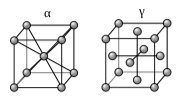
\includegraphics[width=0.45\textwidth]{images/img7.png} 
    \caption{Martensite (dx) e austenite(sx)}
    \labfig{img7}
\end{figure}
\begin{figure}[!hbt]
    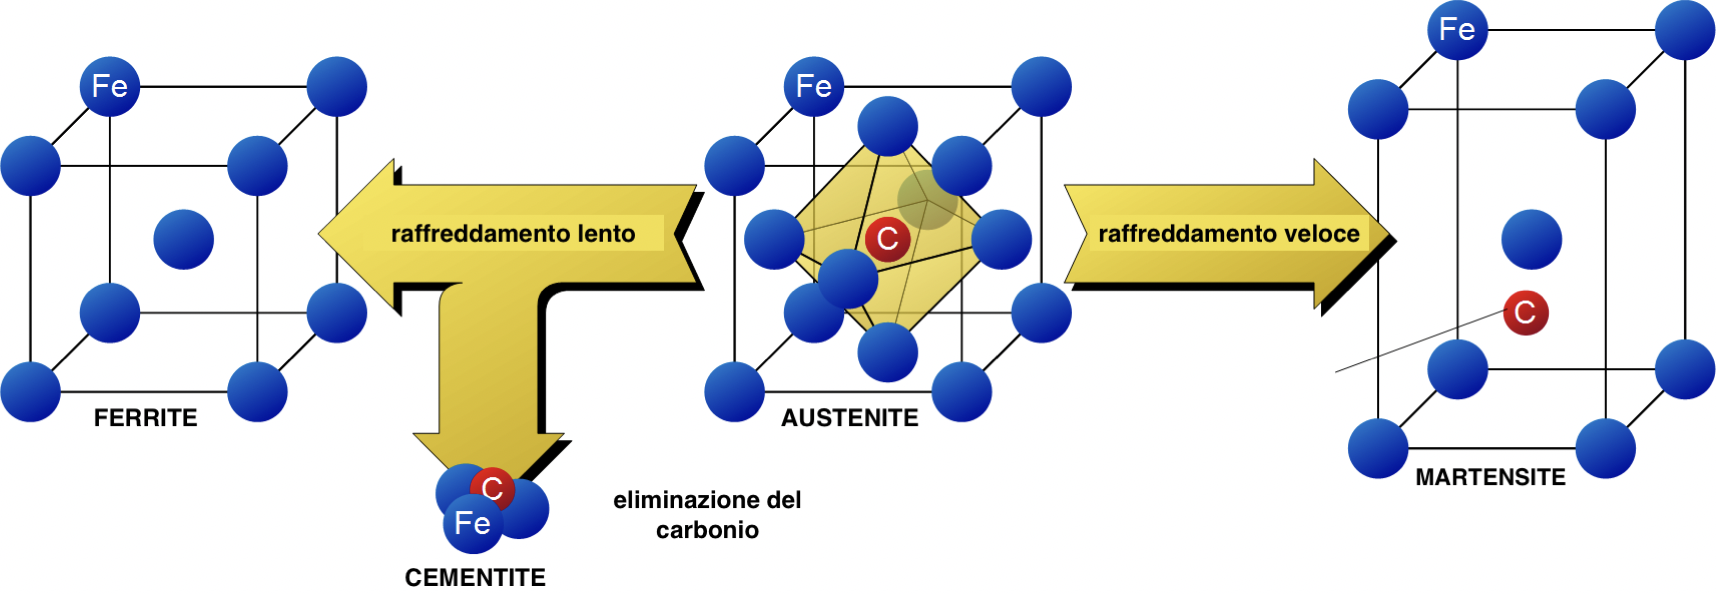
\includegraphics[width=0.65\textwidth]{images/img8.png} 
    \caption{Trasformazione dell'austenite il ferrite o martensite}
    \labfig{img8}
\end{figure}

Durante la saldatura di acciai, si può originare della martensite nella ZTA perché il raffreddamento è troppo rapido: ciò indebolisce il materiale poiché si tratta di una configurazione fortemente tensionata, che non si deforma plasticamente e quindi fragile, molto simile ad un vetro.
La presenza e la quantità di martensite dopo la saldatura, oltre che dalla velocità di raffreddamento, dipende anche dalla composizione chimica dell’acciaio. In realtà, tutti gli elementi, ad eccezione del cobalto, favoriscono la formazione di martensite. Quindi, più l’acciaio è legato, cioè maggiore è la quantità di elementi leganti nella saldatura e nei trattamenti termici, più è facile che si formi martensite e altre fasi metastabili a bassa temperatura. La saldatura risulta difficile e i rischi di frattura sono elevati. La facilità di formazione della martensite è detta temprabilità (si veda sezione \ref{raffreddamento}) ed è in genere favorita dalla presenza di elementi leganti. Si può affermare che \textbf{temprabilità e saldabilità sono inversamente proporzionali}, almeno in prima approssimazione.

Ovviamente, maggiore è la quantità di carbonio intrappolata, tanto più la martensite sarà fragile. Si definisce \textbf{carbonio equivalente}\index{carbonio equivalente} CE:
\begin{equation*}
    \mathrm{C.E. = \%C + \frac{\%Mn}{\alpha} + \frac{\%Si}{\beta} +  \frac{\%Cr+\%Mo+\%V}{\gamma} + \frac{\%Ni+\%Cu}{\delta}}
\end{equation*}
Dove $\alpha,\, \beta,\, \gamma,\, \delta$ sono dei coefficienti fissi che tengono conto della percentuale di martensite che viene creata dai singoli elementi, cioè quantificano l’influenza dell’elemento nella formazione di martensite. C invece è la percentuale di carbonio reale dell’acciaio. Affinché l’acciaio possa essere considerato saldabile, senza incorrere in fratture o rotture, si deve avere C.E. $\le$ 0,4.

La definizione del tenore di carbonio equivalente fa parte dei criteri di saldabilità, insieme alla definizione del tenore inclusionale di zolfo S e fosforo P. Quest’ultimo determina la purezza dell’acciaio.\\
Nel caso di acciai storici, bisogna di tenere in considerazione anche l’uniformità del materiale, effettuando delle prove di trazione e verificando la resistenza del materiale.

Per concludere, affinché una saldatura sia fatta in maniera corretta, possono essere prese diverse precauzioni:
\begin{itemize}
    \item ridurre la differenza di temperatura tra ZTA e bulk, con un pre-riscaldamento del materiale in forno, se possibile (potrebbe non esserlo a causa delle dimensioni). Se bisogna saldare degli stampi, per eventuali modifiche, dato che vi sono alcune zone irrobustite (tallonatura), essi non si possono pre-riscaldare in forno, bensì si utilizza il riscaldamento con cannella o si opta per una saldatura a freddo;
\item coprire la saldatura con materiale inerte (ad esempio con sabbia) che trattiene il calore e rallenta il raffreddamento;
\item prendere le dovute precauzioni affinché si eviti o ci si accorga in tempo di eventuale sviluppo di idrogeno. La formazione di idrogeno è particolarmente dannosa per acciai ad elevata durezza, il che ne rende particolarmente sconsigliata la saldatura.
\end{itemize}

La tecnica più recente di saldatura è la friction stir welding: mentre gli altri metodi consistono nell’apportare direttamente calore, tale tecnica sfrutta l’energia meccanica generata dall’attrito e si usa, ad esempio, per saldare la valvole di un motore sullo stelo.
E’ utilizzata anche nel campo della saldatura dell’alluminio: si mettono i due pezzi a contatto e con una specie fresa, si praticano dei solchi nel materiale, generando attrito e dunque, calore. Tale tecnica non è molto efficace per la saldatura dell’alluminio e dell’acciaio.

Consideriamo un ciclo termico di saldatura: poniamo, in un grafico, sulle ordinate la percentuale di una fase e sulle ascisse il rapporto T/t, detto velocità di raffreddamento, si può vedere che se all’inizio vi è il 100\% di ferrite, con il passare del tempo, tale fase diminuirà e si formerà la martensite. Si nota che, durante tale passaggio, si forma anche un’altra fase metastabile del ferro, detta bainite. Anch’essa, come la martensite, non è una fase di equilibrio e si forma a causa di un raffreddamento troppo veloce: essa rende fragile il materiale e causa la spaccatura della ZTA. Alla fine, si avrà il 100\% di martensite. Il punto di incrocio tra la curva della ferrite e quella della martensite si sposta a velocità di raffreddamento più basse tanto più l’acciaio è legato, cioè per quantità maggiori di carbonio equivalente.

In una saldatura si può avere un doppio pericolo: abbinata alla formazione di martensite, che rende fragile il materiale, si può infatti avere l’idrogenazione, che genera tensioni interne e rottura del materiale nel giunto. Le possibili fonti di idrogeno sono l’umidità, se vi è un materiale non metallico coinvolto nella saldatura, i composti idrati (ruggine) o residui riconducibili a una non corretta pulizia dei lembi dei materiali e l’umidità dell’aria.

L’austenite e la ferrite hanno deformabilità elevata perché hanno poche dislocazioni all’interno dei propri reticoli e quindi, poche tensioni: esse si presentano, infatti, sotto forma di grandi cristalli.\\
Sono più facilmente saldabili gli acciai non temprabili, cioè gli acciai basso legati.
Abbiamo già detto che affinché un acciaio sia considerato saldabile, il carbonio equivalente deve essere minore dello 0,4 \%: si tratta di una condizione necessaria, ma non sufficiente. Invece, per valori superiori allo 0,6\% si ha una saldabilità critica.

Nella produzione di acciaio, gli elementi che non mancano mai, oltre al carbonio C, sono il manganese e il silicio. Inoltre, a causa della composizione del coke, si trovano anche zolfo e fosforo, quindi oltre al carbonio equivalente, è necessario anche valutare il tenore di questi due elementi all’interno dell’acciaio per valutarne la purezza.
Lo zolfo è sempre presente nel carbon fossile, da cui si ricava il metallo; affinché un acciaio sia buono, il tenore di zolfo non deve superare lo 0,01\%. Infatti, lo zolfo ha un’elevata affinità con il ferro e possono formarsi \textit{solfuri di ferro}, che assumono la forma di strisce allungate ben visibili. Questa fase forma un eutettico bassofondente (900-950°C), che non permette di operare lavorazioni termiche dell’acciaio, poiché la temperatura eutettica è la più bassa a cui troviamo il liquido. Inoltre, il solfuro interrompe la matrice metallica rendendo l’acciaio più fragile.
Il processo di eliminazione dello zolfo, detto desolfurazione, è un trattamento molto difficile e costoso e durante la vita dell’acciaio, il tenore di zolfo va sempre monitorato.

\index{acciaio a lavorabilità migliorata}
Esistono però degli acciai, detti acciai automatici o acciai a lavorabilità migliorata, in cui lo zolfo è aggiunto intenzionalmente. La loro caratteristica principale è quella di avere una facile lavorabilità alle macchine utensili ad asportazione del truciolo, cioè sono caratterizzati da una facile truciolabilità. Infatti, quando si lavora un materiale per asportazione di truciolo, il truciolo che si forma si incolla con l’utensile, impastandolo e impedendone il funzionamento. Quando sono necessarie tali lavorazioni, si preferisce un materiale che non produca truciolo o che ne formi uno tale da spezzarsi subito. Si ottiene ciò aggiungendo all’acciaio degli elementi infragilenti, come i solfuri, che creano nel materiale degli intagli a rottura e interrompono la matrice metallica, rendendo la struttura debole.\\
La composizione di questi acciai prevede lo 0,1\% di zolfo, ed è presente anche un alto tenore di manganese maggiore dell’1-1,5\%, mentre negli acciai normali la percentuale di manganese è dello 0,3-0,4\%, al massimo 0,6-0,7\%. Infatti, manganese e zolfo sono molto affini e reagiscono fra loro, formando solfuri di manganese, e non solfuri di ferro, che hanno un eutettico (si veda capitolo \ref{Fe-C}) a 1200-1250 °C\sidenote{L'eutettico del solfuro di ferro si aggira intorno ai 900°, che è una temperatura pericolosamente vicina a quella di austenitizzazione. Questo comporta il rischio di generare una fase liquida durante il riscaldamento.}. Grazie a questo accorgimento si possono operare trattamenti termici, conservando la caratteristica di fragilità. Quindi, il solfuro di manganese è necessario in qualsiasi tipo di acciaio che ha necessità di essere lavorato molto facilmente. Ad esempio, le viti delle sedie sono fatte di acciai automatici: esse sopportano uno sforzo praticamente nullo, quindi non importa che siano fragili, ma devono essere maschiate, cioè lavorate con una macchina utensile ad asportazione di truciolo. Quindi, si usa lo zolfo per migliorare la truciolabilità e il manganese per alzare la temperatura eutettica.

Una volta gli acciai non erano al manganese-zolfo, bensì al piombo, in quanto esso non si scioglie nel ferro: si gettavano dei pallini da caccia in piombo, cioè delle microsfere, che rimanevano intrappolati nell’acciaio, indebolendo e autolubrificando la struttura, migliorando la lavorabilità dell’acciaio. Si è abbondata questa tecnica sia perché il piombo non è benefico per la salute umana (avvelenamento da piombo) sia perché il piombo è un elemento molto più pesante del ferro e quindi, durante la solidificazione dell’acciaio, rischia di finire sul fondo del getto rendendo la sua distribuzione non uniforme.

Durante la saldatura si possono formare dei difetti, come le cricche a caldo e cricche a freddo, che si formano durante la fase di raffreddamento per le tensioni viste in precedenza. Altri difetti possono essere porosità dovute dalla presenza di idrogeno, argon e azoto.

Abbiamo visto che gli acciai inossidabili non possono arrugginire. Tuttavia, se si utilizzano acciai inox automatici, per aumentare la truciolabilità, i solfuri di manganese e l’austerità formano la cosiddetta pila di corrosione e l’acciaio non è più inossidabile.

\section{Raggi X}
\subsection{Teorie atomiche}

Sin dall’antichità si credeva che la materia fosse costituita da elementi piccolissimi e indivisibili (a- tomo, dal greco, significa non divisibile), cioè tutta la particella conserva le caratteristiche della materia. \\
Per primi i raggi X misero in dubbio l’indivisibilità dell’atomo e portarono alla scoperta di neutroni, elettroni e protoni.\\
Il primo che scoprì la divisibilità dell’atomo fu Thomson, il quale inserì in un’ampolla un anodo e un
catodo producendo una scarica elettrica di gas rarefatti: osservò che il raggio si divideva in due sottragga diversi e ciò significava che esistevano componenti positivi e componenti negativi della materia. In seguito, studiando l’andamento dei due raggi al variare del campo magnetico alla quale erano sottoposti, \textbf{Thomson} capì che le cariche negative pesavano molto meno. Nacque, così, il modello a panettone dell’atomo.\\
Anche Rutherford scoprì che, sparando delle particelle $\alpha$, cioè elio senza elettroni, su lamine di oro, che è molto malleabile: la maggior parte delle particelle attraversavano l’atomo e solo alcune rimbalzavano. Egli pensò che l’atomo fosse costituito da vuoti e che la materia fosse posizionata solo in alcuni punti con carica positiva. Poiché più cariche positive a contatto si respingerebbero, esse interagiscono con i neutroni, mentre gli elettroni si muovono su orbite circolari.
Per Keplero, tali orbite erano ellittiche, come quelle dei pianeti nel sistema solare.\\
Tuttavia la teoria di \textbf{Rutherford} non spiegava come fosse possibile che una particella in movimento, l’elettrone, perdendo energia non collassare sul nucleo. La differenza fra pianeti ed elettroni è che nel prima caso vi è attrazione gravitazionale, nel secondo attrazione elettrostatica: quindi una carica elettrica in movimento in un campo elettromagnetico perde energia cinetica, che diventa elettromagnetica, ma comunque la particella non collassa sul nucleo.\\
Entra, quindi, in gioco \textbf{Bohr}, il quale applicò alla propria teoria le scoperte di \textbf{Planck}. Fino ad allora si era abituati a vedere l’evoluzione dei fenomeni in modo continuo: infatti, come afferma Lucrezio nel “De rerum natura”, “natura no facit salti”, cioè la natura non fa salti. Invece, Plack, studiando la luce, scoprì che una lampadina non emette un raggio continuo di luce, bensì luce sotto forma di pacchetti di energia, chiamati in generale quanti e nello specifico fotoni.\\
Bohr capì che il fenomeno di Thomson era giustificabile con la teoria dei quanti di Planck: egli divise lo spazio intorno all’atomo in vari livelli di energia e l’elettrone, che possiede energia, può trovarsi solo in un livello energicamente ad esso concesso. Finché rimane in uno specifico livello, l’energia dell’elettrone non cambia. Per far salire di livello un elettrone, bisogna fornirgli l’energia necessaria ad effettuare il salto. Si arrivò, così, al modello atomico di Bohe, con l’uso di quattro numeri quantici.\\
Tuttavia, la teoria non era ancora perfetta poiché si insisteva nell’applicazione della fisica classica per determinare la posizione degli elettroni negli orbitali. Tuttavia l’elettrone si muove lungo distanze interatomiche dell’ordine di 1 Å con una velocità prossima a quella della luce di 300000 km/s: misurando la sua posizione si commette un errore infinitamente superiore alla misura stessa. Si inizi, quindi, a ragionare in termini probabilistici, definendo l’orbitale come il luogo dopo con maggiore probabilità si trova l’elettrone dal punto di vista energetico: risolvendo l’equazione di Schrödinger si trovano tali orbitali.

\subsection{Raggi X: corpo umano e materiali metallici}

Si può instaurare un parallelismo fra il corpo umano e i materiali metallici. Le analisi che si fanno al corpo umano esistono in modo equivalente per i materiali metallici: ad esempio, le analisi del sangue sono le analisi chimiche del materiali oppure i raggi X delle lastre sono gli stessi usati per studiare la struttura interna di un materiale metallico. Tale analisi prende il nome di \textbf{analisi roentgenografica}.

I raggi X si generano in un tubo in cui è presente una grossa lampadina: il filamento della lampadina, essendo percorso da corrente, si scalda ed emette elettroni, che, accelerati da un campo magnetico esterno, collidono con una placchetta di metallo, detta anticatodo, posta alla fine del tubo.
La potenza dei raggi X dipende sia dal valore della corrente sia da quello della differenza di potenziale.

L’atomo è costituito da un nucleo, formato da neutroni e protoni, ed elettroni, i quali hanno 1/1840 della massa del protone. Secondo la meccanica quantistica, gli elettroni si possono muovere in zone, chiamate orbitali, a loro energicamente concesse, cioè con energia simile.
Per descrivere questa situazione si ricorre a numeri quantici:
\begin{itemize}
    \item il primo numero quantico (\textbf{n}) individua in che livello energetico èsituato l'elettrone;
    \item il secondo numero quantico (\textbf{l}) individua il tipo di orbitale;
    \item il terzo numero quantico ($\mathrm{\bold{m_l}}$) individua il numero di orbitali (1 orbitale sferico, 3 orbitali a forma di 8, 5 orbitali d);
    \item il quarto numero quantico individua lo \textbf{spin}. Essendoci in un orbitale massimo due elettroni, essi hanno spin antiparalelli (\textbf{principio di esclusione di Pauli}).
\end{itemize}

Queste conclusioni furono fatte da Bohr e Sommerfield, partendo dalle ipotesi di Rutherford, il quale sosteneva che gli elettroni si muovessero su orbite ellittiche. Bohr, invece, mutuò dalle teorie di Planck il modello della discrezione energetica. Planck, infatti, descrisse i fenomeni luminosi non come continui, ma come un’emissione di pacchetti di energia infinitesimi, i fotoni, che dall’uomo vertono percepiti continui. I fenomeni energetici vengono descritti, ciò, come una scalinata con dei salti.

Non si può dire con certezza dove si trovi un elettrone, in quanto muovendosi con la velocità della luce (300000 km/s) in distanze interatomiche quali l’Angstrom ($10^{-10}$ m), l’errore commesso sulla misura è infinitamente maggiore della misura stessa. Con l’equazione di Schrödinger, gli orbitali diventano la regione in cui si ha la massima probabilità di trovare gli elettroni, ed essi possono cambiare orbitale quando cambia il loro livello energetico.\\
Comunemente, però, l’orbitale viene considerato il luogo dove sono posizionati gli elettroni.

I raggi X sono generato in un tubo, immerso nel vuoto per evitare la corrosione, contenente una grossa lampadina, costituita da un filamento di tungsteno, percorso da corrente che, scaldandosi, emette elettroni per effetto termoionico, e da una placchetta di metallo, detta anticatodo, fatta di tungsteno, di ferro, di rame o di cobalto. Il vuoto del tubo è necessario sia perché il filamento incandescente, che ha una propria resistenza, brucerebbe in presenza di ossigeno, sia perché gli elettroni e- sarebbero fermati dall’aria stessa.\\
Il sistema è immerso in un campo magnetico che accelera gli elettroni verso l’anticatodo, che è il polo positivo.\\
Entrando in contatto con l’anticatodo, l’elettrone collide con esso e viene frenato, o addirittura fermato, e la sua energia elettro-cinetica in parte si trasforma in calore (circa 99\%), in parte viene trasformata in radiazioni (circa 1\%), cioè i raggi X. Proprio a causa dell’elevato calore che viene sviluppato, i tubi devono essere raffreddati (anche l’acqua può essere usata come refrigerante). Le radiazioni sono prodotte in tutto il volume del tubi, ma essi sono schermati e di solito, presentano quattro apertura, di cui solo una è attiva.\\
Dato che l’energia cinetica posseduta dall’elettrone diminuisce, cioè decelera, l’energia delle radiazioni emesse sotto forma di raggi X è variabile.

L'energia di radiazione è uguale alla costante di Planck ($h$) per la sua frequenza ($\nu$): $\mathrm{E}=h\nu$.\\
Si definisce rumore di fondo l’insieme di radiazione di energia non ben definita, cioè di diverse lunghezze d’onda, ma costituenti un unico pacchetto di energia. Infatti, il rumore di fondo è definito come una somma di oscillazioni irregolari, intermittenti o statisticamente casuali.


Come già detto, l’intensità del fascio di radiazioni dipende dall’intensità di corrente [mA]: il numero di elettroni liberati dal filamento è, infatti, proporzionale ad essa. Per variare la quantità di elettroni bisogna, quindi, variare la corrente: aumentarla significa aumentare la temperatura e conseguentemente, vi è un aumento della resistenza R del filamento per effetto Joule, quindi vi è un aumento della quantità di elettroni emessi.\\
La qualità del fascio determina il potere penetrante della radiazione e dipende dall’energia degli elettroni emessi dal filamento, che a sua volta dipende dalla differenza di potenziale [kV]: maggiore è la differenza di potenziale, maggiore sarà l’energia degli elettroni.

I raggi X attraverso la materia in modo proporzionale alla loro energia: gli elettroni, infatti, possono interferire con la materia, quindi essere assorbiti durante il loro passaggio oppure essere semplicemente frenati. Il rallentamento dipende dal tipo di materiale e dello spessore della lastra: il piombo, ad esempio, è usato per schermare.

Avendo i raggi X una lunghezza d'onda paragonabile alle distanze interatomiche possono interagire in maniera particolare con la materia solida. In particolare sono in grado di attraversarla, entro certi limiti di spessore\sidenote{Nelle applicazioni mediche di usano radiazioni ad elevata penetrazione}. La luce visibile, ad esempio, non è in grado di fare prodezze del genere, perché presenta lunghezze d'onda molto maggiori.

La potenza dei raggi X è influenzata da due parametri: l’intensità di corrente, misurata in mA, determina la quantità di elettroni emessi, e la differenza di potenziale, misurata in kV, determina il potere penetrante.\\
Per i materiali metallici, si utilizzano correnti di 20-30 mA e voltaggi di circa 40 kV, mentre per usi medici, le correnti hanno intensità simili alle precedenti (non possono essere troppo elevate perché si rischia di bruciare il filamento di tungsteno), ma i voltaggi sono di circa 100-150 kV.

I raggi X vengono generati nel cosiddetto \textbf{tubo di Coolidge}, che è costituito da una lampadina e da un anticatodo. Se vi è solido interposto tra i raggi X e l’ambiente esterno, esso assorbe i raggi X, totalmente o parzialmente, e una lastra posta dietro il corpo sarà impressionata in maniera differente a secondo che ci sia o meno materia. I punti del materiali hanno diverse reazioni di fotosensibilizzazione.

Dal punto di vista medico, i raggi X si utilizzano per determinare la rottura di un osso: infatti, esso viene messo in evidenza poiché l’osso assorbe radiazioni, quindi apparirà bianco sulla lastra, mentre dove vi è la frattura, la radiazione passa indisturbata e apparirà una zona nera sulla lastra.\\
Dal punto di vista metallurgico, un acciaio, ad esempio, impressionerà una lastra in maniera diversa in base alla fase presente (ferrite, austenite).
I raggi X possono far vedere cosa accade dentro il materiale senza dover fisicamente aprire il pezzo, cioè permettono di effettuare prove non distruttive. Essi si utilizzano, ad esempio, per verificare che il catalizzatore sia ben distribuito nella marmitta, per individuare scorie, porosità, bolle, inclusioni, soffiature, incollaggi nel cordone di saldatura: tali difetti assorbono le radiazioni diversamente e possono così essere individuati all’interno del materiale.
I raggi X sono impiegati per individuare i difetti sub-superficiali: non riescono, infatti, a penetrare un grande lingotto (carro armato) oltre la superficie.

I difetti che si rilevano con i raggi X dipendono sia dalla posizione dell’oggetto rispetto ai raggi sia dal potere penetrante delle radiazioni.
Considerando la posizione dell’oggetto in base all’orientamento del difetto, si ha che l’evidenziazione di quest’ultimo sarà tanto maggiore quanto minore è la quantità di materia intercettata. Prendiamo come esempio una cavità cilindrica: se l’oggetto è perpendicolare ai raggi X, il potere assorbente è molto piccolo; se l’oggetto è parallelo ai raggi X, il potere assorbente è molto elevato.\\
Invece, il potere penetrante dei raggi X è limitato e dipende dal materiale attraversato, cioè non riescono ad attraversare grandi spessori. Il corpo umano, ad esempio, è costituito dal 70\% di acqua e quindi i tessuti molli sono facilmente penetrabili dai raggi X.\\
Nei metalli, invece, la quantità di radiazione assorbita dipende dalla fase e dal tipo di materiale: il piombo è poco penetrabile; l’austenite e la ferrite hanno potere assorbenti diversi.\\
Quindi, affinché un difetto possa essere ben evidenziato, è necessario valutare la profondità del difetto e l’orientamento favorevole dei raggi X.

Spesso, per verificare la corretta della prova, il materiale da analizzare è affiancato da un cuneo costituito dallo stesso materiale. Il cuneo è un oggetto a spessore variabile, e grazie a questa forma si può tarare la radiazione per capire a quale profondità si trova il difetto: i raggi X impressioneranno la lastra in maniera differente in base allo spessore che hanno dovuto percorrere.

Esistono anche i \textbf{raggi} $\boldsymbol\gamma$, molto più penetranti dei raggi X, poiché essi si originano dal decadimento degli elementi radioattivi. Essi, però, sono molto meno utilizzati in quanto meno gestibili: se la sorgente di raggi X può, infatti, essere spenta per essere utilizzata solo nel lasso di tempo necessario, il decadimento continua nel tempo. E’ necessario utilizzare molte precauzioni ed operare in luoghi protetti, poiché si è in present di una sorgente radioattiva sempre attiva.
Inoltre, i raggi $\gamma$ sono molto pericolosi in quanto possiedono una grandissima energia e possono apportare anomalie nel corpo umano, in particolare nel funzionamento e nella riproduzione delle cellule (tumori).

\subsection{Spettro dei raggi X}

Lo spettro dei raggi X può essere rappresentato come la distribuzione dell’energia totale dei fotoni X prodotti in funzione della loro energia al variare della tensione di alimentazione di picco del tubo.\\
Lo spettro dei raggi X presenta una caratteristica curva, detta \textit{Bremsstrahlung}, detta anche radiazione di frenamento o di fondo, definita come la radiazione emessa da particelle cariche quando subiscono una decelerazione. Ciò avviene per esempio quando le particelle vengono scagliate contro un bersaglio metallico. Poiché gli elettroni sono molto più leggeri dei protoni (massa a riposo circa duemila volte inferiore) il bremsstrahlung degli elettroni è la più comune; infatti l'intensità delle onde emesse è inversamente proporzionale al cubo della massa.

\begin{figure}[hb]
    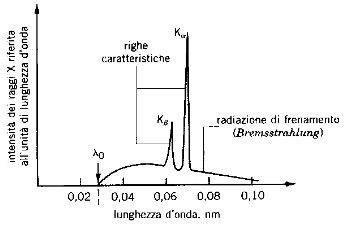
\includegraphics[width=0.6 \textwidth]{images/img9.jpg}
    \caption{Spettro di emissione dei raggi X.}
    \labfig{img9}
\end{figure}

La curva non parte da zero: vi è infatti una lunghezza d’onda minima, $\lambda_{min}$, che dipende dalla differenza di potenziale, e rappresenta l’energia cinetica degli elettroni: $\mathrm{E_c}=hc/\lambda_{min}$. Infatti, l’energia cinetica degli elettroni è definita come il prodotto fra la carica dell’elettrone e la differenza di potenziale a cui è sottoposto: $\mathrm{E_c = e^-\Delta V}$.
La radiazione di bremsstrahlung è caratterizzata da una distribuzione continua di radiazione che diviene più intensa e si sposta verso le frequenze maggiori con l'aumentare dell'energia degli elettroni bombardanti. La frequenza massima della radiazione è legata all'energia cinetica degli elettroni da $\mathrm{E_c}= hc/\lambda_{max}$.

La radiazione di fondo corrisponde a un certo pacchetto di frequenze.
Gli elettroni, oltre a cedere energia sotto forma di radiazioni e di calore, la cedo anche agli elettroni dell’anticatodo, che acquistando un’energia, cioè un pacchetto energetico ben preciso, saltano ad un livello superiore (come afferma la teoria di Planck). Quando l’effetto finisce, gli elettroni dell’anticatodo avranno un’energia inferiore a quella richiesta dal livello in cui si trovano e sono costretti a tornare al livello iniziale, rilasciando, però, l’energia in eccesso sotto forma di radiazioni con una specifica lunghezza d’onda, che è rappresentata nel grafico come un picco. Quindi, gli elettroni dell’anticatodo sono tornati al loro livello energetico iniziale, rilasciando pacchetti di energia ben precisa e proporzionale alla lunghezza d’onda $\lambda$. Si ottiene così un secondo tipo di raggi X.

Si possono quindi scegliere due strade diverse nella selezione delle radiazioni:
\begin{enumerate}
    \item si utilizzano indistintamente tutte le lunghezze d’onda, come nel caso della macroscopia (macrodiffrazioni - roentgenografia), cioè per usi medici\sidenote{principio di assorbimento delle radiazioni ad opera della materia};
    \item si utilizzano solo i picchi, cioè radiazioni emesse dall’anticatodo con lunghezze d’onda ben definite\sidenote{fenomeno della diffrazione}.
\end{enumerate}

Ogni materiale ha un suo spettro caratteristico, in quanto lo spettro di un materiale corrisponde alla sua impronta digitale, e attraverso di esso, si può procedere con un’analisi chimica del materiale.

Molto importanti sono gli spettri di fluorescenza o di emissione, che vengono ricavati attraverso la tecnica della \textbf{spettrofotometria XRF} (X-ray fluorescence spectroscopy o X-ray fluorescence): si tratta di una tecnica di analisi non distruttiva che permette di conoscere la composizione elementale di un campione attraverso lo studio della radiazione di fluorescenza X. Tale radiazione è emessa dagli atomi del campione in seguito a eccitazione (che può dare anche effetto fotoelettrico), che si ottiene tipicamente irraggiando il campione con raggi X e gamma ad alta energia.
L’isotopo $\mathrm{^{109}\mathrm{Cd}}$ è spesso usato come sorgente di raggi X a 214 keV.
Due strumenti utili per l’analisi di un materiale sono il \textbf{microscopio ottico} e il \textbf{microscopio elettronico}. Quest’ultimo può essere utilizzato per un’analisi della morfologia superficiale del materiale, sfruttando la collisione fra gli elettroni e un conduttore metallico e ricreando su un monitor lo spettro di un materiale. Se si abbina al microscopio anche una microonda, è possibile ottenere un’analisi puntuale del materiale.

La spettroscopia EDX (Energy Dispersive X-ray Analysis) o spettroscopia EDS (Energy Dispersive X-ray Spectrometry) è un metodo analitico strumentale che sfrutta l'emissione di raggi X generati da un fascio elettronico accelerato, incidente sul campione. La strumentazione è comunemente costituita da un microscopio elettronico a scansione. Schematicamente si può descrivere il principio di funzionamento nel seguente modo: un emettitore costituito da un filamento di tungsteno, che viene portato oltre i 1000 °C per riscaldamento elettrico, funge da sorgente di elettroni per effetto termoionico. Il fascio elettronico così generato viene accelerato da una differenza di potenziale di 0,3-30 KV e costretto a passare prima attraverso un collimatore elettromagnetico per essere deflesso, in modo da generare la scansione, e successivamente collimato verso il piatto contenente il campione in esame. Tutto ciò è svolto sotto vuoto, a circa 10-5 mbar, per aumentare il libero cammino medio degli elettroni ed evitare fenomeni di diffusioni a causa di interazioni aria-elettrone.\\
Il rivelatore, che è disposto in modo tale da ricevere il massimo livello di radiazione assorbibile, può essere del tipo \textbf{a dispersione di lunghezza d'onda} (WDS - Wavelength-dispersive X-ray spectroscopy) o \textbf{a dispersione di energia} (EDS - Energy-dispersive X-ray spectroscopy):
\begin{itemize}
    \item il rivelatore \textbf{WDS} sfrutta le caratteristiche ondulatorie dei fotoni X. È costituito da un cristallo
ricurvo, il "cerchio di Rowland", con un determinato passo d del reticolo cristallino, sul quale sono disposti il campione e il contatore di fotoni. Seguendo la legge di Bragg, solamente una determinata lunghezza d'onda sarà riflessa sul contatore, lunghezza d'onda che può essere variata ruotando il rivelatore. Quindi, tale metodo è utilizzato per contare il numero di raggi X di una determinata lunghezza d’onda diffratti da un cristallo.
\item il rivelatore \textbf{EDS} sfrutta l'interazione energetica tra i raggi X e un opportuno materiale. Tale
rilevatore è utilizzato per l’analisi chimica del campione in esame, che è principalmente influenza dalla struttura atomica di quest’ultimo e dal suo spettro di emissione. È caratteristicamente rappresentato da un monocristallo di silicio drogato con litio, rivestito alle due estremità con uno strato conduttivo in oro, mantenuto in alto vuoto e alla temperatura di -192 °C con azoto liquido. Il cristallo di germanio ad elevata purezza rappresenta una moderna evoluzione più efficiente. Il principio di funzionamento sfrutta la produzione di corrente elettrica, che viene sensibilmente amplificata, generata per interazione tra fotoni e cristallo. Sono i rivelatori attualmente più utilizzati.
\end{itemize}

\subsection{Diffrazione e cristallografia}

Nel 1912 Von Laue ipotizzò che il reticolo cristallino si comportasse come un reticolo di diffrazione con i raggi X e scoprì la diffrazione dei raggi X da parte dei reticoli cristallini.

In un reticolo cristallino, gli atomi sono disposti secondo sequenze geometricamente ben definite (cubica, esagonale, tetragonale, monoclina, etc) e ripetibili. Ad esempio, il vetro non è un solido cristallino, ma è amaro, cioè il cosiddetto “liquido solidificato”. Infatti, nei liquidi, gli atomi assumono posizioni del tutto casuali poiché sono liberi di muoversi. Quasi il 100\% dei materiali metallici è un solido cristallino.

La diffrazione dei raggi X è una delle tecniche più importanti per lo studio dei solidi cristallini. Qualunque radiazione elettromagnetica è in grado di interagire con la materia attraverso due processi principali:
\begin{itemize}
    \item \textbf{assorbimento}: nel corso del quale la radiazione cede tutta o parte della propria energia al
sistema materiale, aumentandone la temperatura o determinandone la transizione ad uno stato eccitato. Nel caso dei raggi X, la radiazione incidente ha energia sufficiente per provocare transizioni elettroniche, ed espellere elettroni dagli atomi (effetto fotoelettrico). Si utilizzano gli spettri di assorbimento in campo medico;
\item\textbf{diffusione} (scattering): nel corso del quale la radiazione viene diffusa dalla materia e le onde elettromagnetiche ad essa associate cambiano direzione di propagazione. Tale cambiamento può essere accompagnato da scambio di energia tra fotoni e materia (scattering anelastico; scattering termico diffuso) o no (scattering elastico).
\end{itemize}

La tecnica della diffrazione di raggi X si basa sullo scattering elastico coerente: il fenomeno macroscopico della diffrazione nasce, infatti, dalla \textbf{somma coerente di tutte le onde elettromagnetiche} diffuse dagli atomi che si trovano lungo una stessa famiglia di piani reticolari. Per manifestarsi, richiede necessariamente la presenza di un ordine a lungo raggio, come si riscontra nei cristalli.

Le tecniche strumentali della diffrattrometria a raggi X forniscono le seguenti informazioni:
\begin{itemize}
    \item caratteristiche dell'unità di ripetizione del reticolo cristallino di una sostanza, cioè le \textbf{costanti reticolari};
    \item \textbf{gruppo spaziale della sostanza}: ioè gli elementi di simmetria puntuali e traslazionali del cristallo;
    \item connettività chimica dell'\textbf{unità asimmetrica}, cioè la più piccola unità strutturale che nessuna operazione di simmetria del cristallo, tranne l'identità, può rimandare in sé stessa. Nel caso dei cristalli molecolari (cioè le cui unità di ripetizione sono molecole), il più delle volte l'unità asimmetrica coincide con la singola molecola, ma non è escluso che possa comprendere due o più molecole, o addirittura una frazione di molecola;
    \item \textbf{moto termico degli atomi o ioni}.
\end{itemize}

Questa analisi si effettua tramite un \textbf{monocromatore}, che è essenzialmente un filtro che permette ad una sola radiazione, cioè ad un solo colore, di uscire dal tubo di Coolidge, tipicamente quella corrispondente al primo picco, cioè $\mathrm{K_{\alpha}}$. Infatti, la luce può essere scomposta in diverse radiazioni caratterizzate ognuna da una specifica lunghezza d’onda e quindi, da specifici colori.\\
Dal monocromatore uscirà una radiazione con una lunghezza d’onda, dell’ordine di 10-10 m, e un’energia ben definite (\textbf{microrontgenografia}). Solo in tali condizioni è possibile il fenomeno della diffrazione. Infatti, la luce non può penetrare i materiali poiché la sua lunghezza d’onda è molto maggiore delle distanze interatormiche: $\mathrm{\lambda_{luce}\approx 10^{-9} > \lambda_{atomiche}\approx 10^{-10}}$.


Lo strumento che comprende monocromatore ed altri strumenti utili all’analisi si chiama \textbf{diffrattometro}.\\
I raggi che incidono sul campione posso essere considerati paralleli perchè la sorgente si può considerare posta ad una distanza praticamente infinita dal campione stesso: $10^{-2} \mathrm{m} \gg 10{-10}$ m. Inoltre, per una semplificazione ingegneristica, assumiamo che i raggi X si comportino come raggi luminosi riflessi (in realtà, i raggi X che penetrano il materiale vengono riemessi, quindi riflessi, dal materiale stesso).\\
Vi è poi un \textbf{contatore}, cioè uno strumento che in grado di intercettare le radiazioni che vengono riemesse, ottenendo un segnale.\\
Le radiazioni diffratte avranno in generale una fase differente e il segnale sarà massimo se sono in fase, mentre sarà minimo (o addirittura nullo) se si trovano in opposizione di fase.

Per ipotesi, assumiamo che le radiazioni che incidono il primo piano siano perpendicolari fra al piano, cioè l’angolo di incidenza sia molto grande, e siano tutte in fase, perché parallela fra loro.
\begin{figure}[hb]
    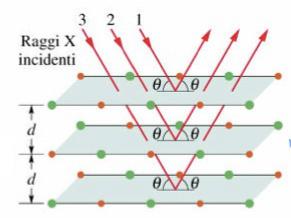
\includegraphics[width=0.6\textwidth]{images/img10.png}
    \caption{Schema della diffrazione dei raggi X attraverso un reticolo cristallino.}
    \labfig{img10}
\end{figure}

Dopo essere stati diffratti, per avere ancora radiazioni in fase, è necessario che la differenza di cammini ottici sia pari ad un numero intero di lunghezze d'onda, secondo la \textbf{legge di Bragg}:
\begin{equation*}
    \mathrm{m\lambda = 2d\sin{\theta}\quad con\, m\in\mathbb{N}}
\end{equation*} 
dove:\begin{itemize}
    \item d è la costante geometrica del reticolo;
    \item $\lambda$ è la lunghezza d'onda;
    \item $\theta$ è l'angolo di incidenza
\end{itemize}
La legge di Bragg può essere facilmente ottenuta considerando le condizioni necessarie per ottenere la fase dei raggi coincidente, cioè quando l'angolo d'incidenza è uguale all'angolo di riflessione. I raggi del fascio incidente sono sempre in fase e paralleli fino al punto nel quale il raggio superiore incontra lo strato superiore dell'atomo z. Il secondo raggio continua fino al successivo strato dove è diffratto dall'atomo B. Il secondo raggio deve attraversare una distanza maggiore AB + BC se i due raggi devono continuare a viaggiare adiacenti e paralleli.
Questa distanza extra deve essere un multiplo intero della lunghezza d'onda ($\lambda$) affinché la fase dei due raggi sia la stessa: n$\lambda$ = AB + BC e poiché AB = BC, si avrà n$\lambda$ = 2AB. Riconoscendo d come l'ipotenusa del triangolo rettangolo Abz, si può usare la trigonometria per mettere in relazione d e $\theta$ con la distanza $AB+BC: AB = d \sin\theta$. Sostituendo tale nell'equazione precedentesi ottiene: $\mathrm{n\lambda = 2 d} \sin{\theta}$.

\begin{marginfigure}[-5cm]
     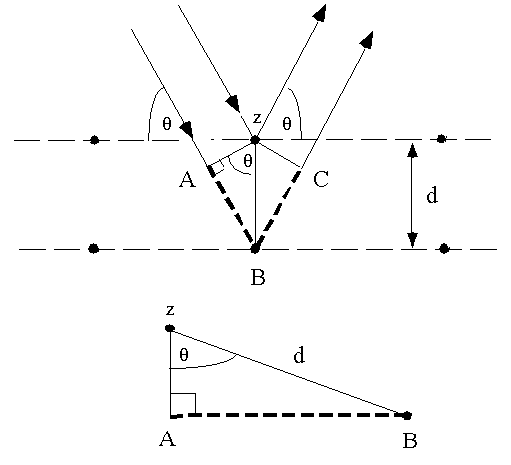
\includegraphics{images/img11.png}
     \labfig{img11}
\end{marginfigure}

Il cristallo è montato su un porta-campioni che lo fa ruotare lentamente in modo da portare tutti i raggi riflessi nelle condizioni di diffrazione, cioè si fa variare l’angolo $\theta$, mantenendo fissa la lunghezza d’onda $\lambda$.\\
L’intensità delle radiazioni emesse viene misurata tramite un contatore Geiger, che dovrà ruotare in sincronismo con il campione per intercettare i raggi. Esso ruota su una circonferenza il cui centro è proprio il campione e la sua velocità angolare $\Phi$ deve essere doppia rispetto a quella del campione $\Psi$, poiché l’angolo alla circonferenza spazzato dal contatore è la metà dell’angolo al centro spazzato dal campione: $\Phi$ = 2$\Psi$. Per questo motivo, sulle ascisse vi è l’angolo 2$\theta$.
\begin{marginfigure}[-5.5cm]
     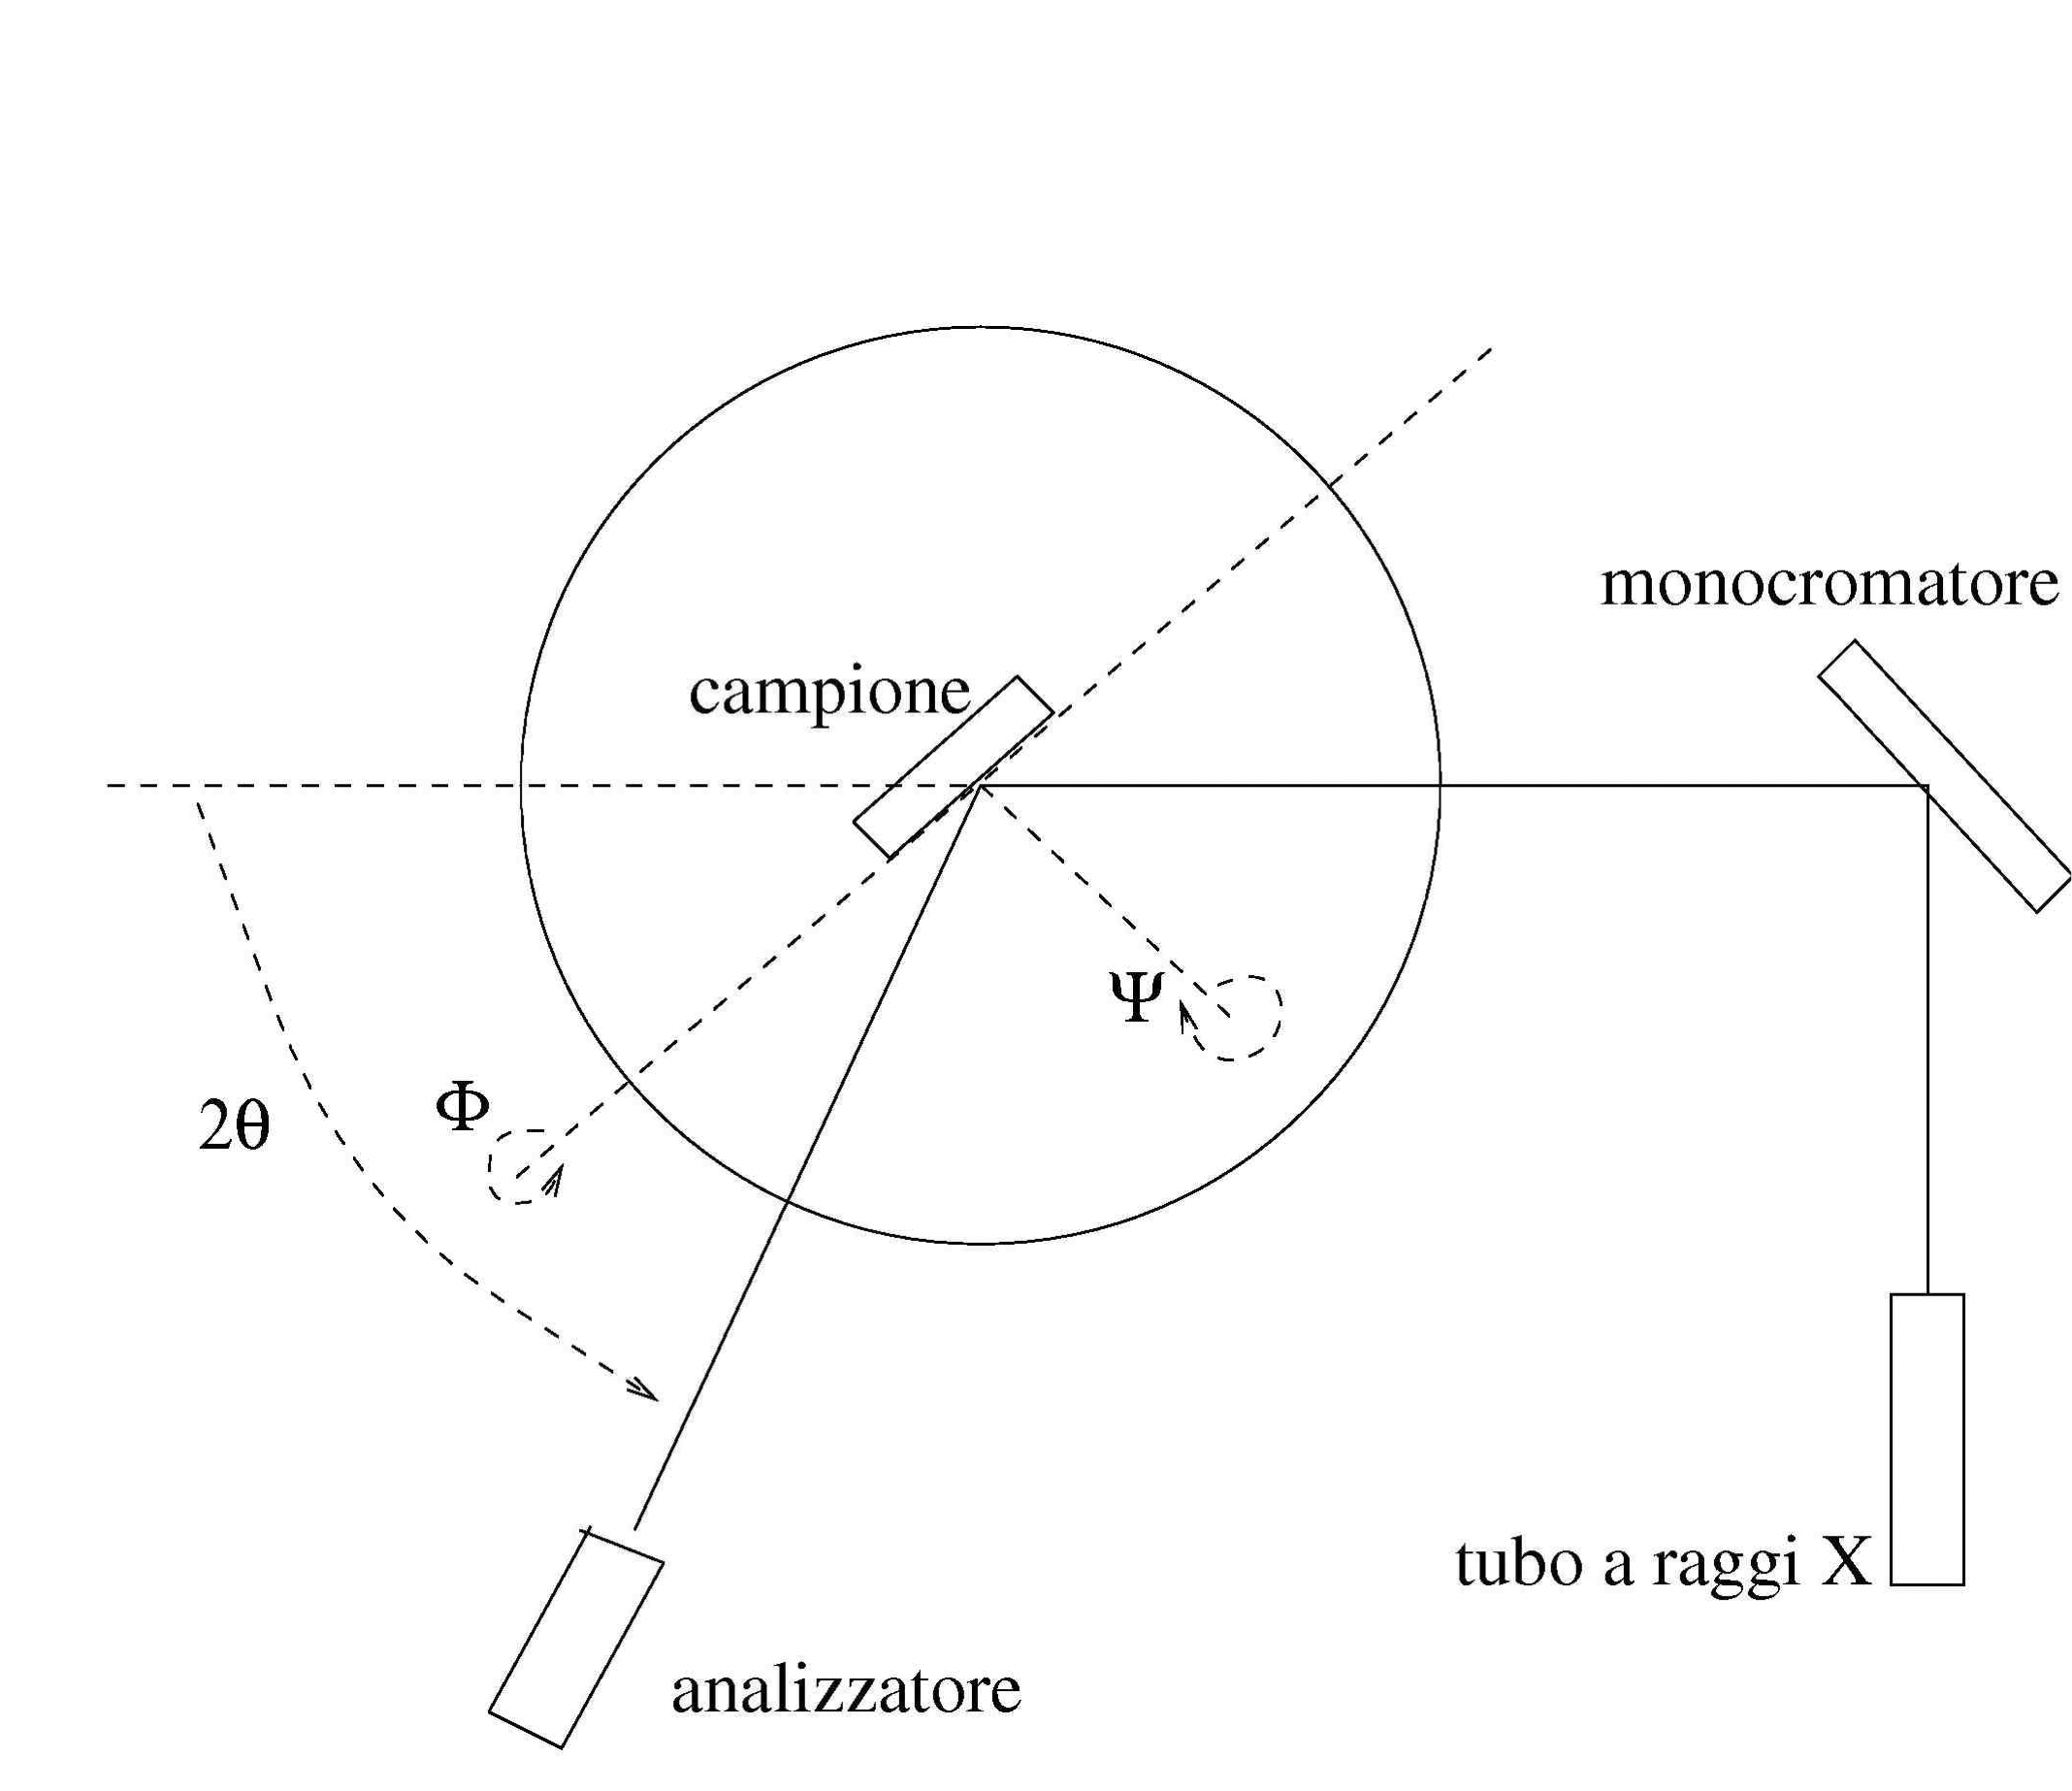
\includegraphics{images/img12.png}
     \caption{Schema di funzionamento di un contatore Geiger}
     \labfig{img12}
\end{marginfigure}
Si ottiene, così, il \textbf{reticolo di diffrazione}, in cui si registreranno una serie di picchi, che indicano tutte le volte che è stata rispettata la legge di Bragg.\\
Cambiando le condizioni di funzionamento, cioè modificando la radiazione, il diagramma si sposterà: esso, quindi, dipende dalla lunghezza d’onda $\lambda$ e dall’angolo di incidenza $\theta$, ma non dalla distanza dai piani d poiché è fissa.
Dunque, è necessario prima di leggere il grafico conoscere la radiazione che l’ha prodotto.
\begin{figure}[hb]
    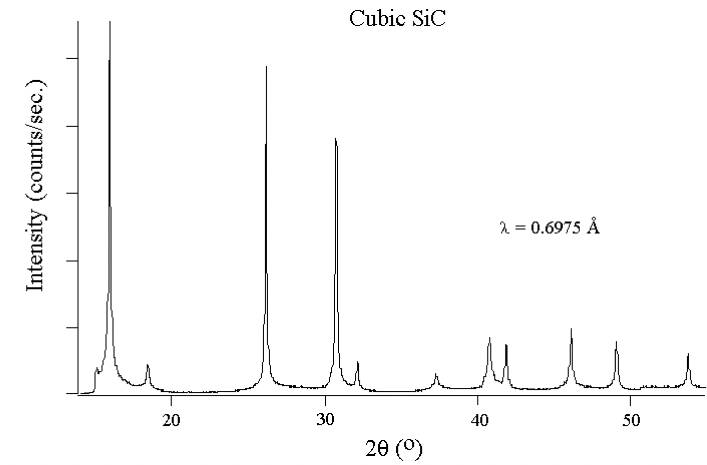
\includegraphics[width=0.6\textwidth]{images/img13.png}
    \caption{Reticolo di diffrazione del SiC cubico }
    \labfig{img13}
\end{figure}

Alcuni sistemi non utilizzano una radiazione monocromatica, bensì una radiazione bianca, e non mettono il campione in rotazione, cioè l’angolo $\theta$ è fisso, ma varia la lunghezza d’onda $\lambda$.

Assumendo come strumento di analisi un monocromatore, $\lambda$ è noto poiché la radiazione viene scelta, $\theta$ misurato dallo strumento, e quindi, è possibile ricavare la costante reticolare d.
Quando si ottiene lo spettro di una sostanza, per leggere correttamente il grafico si effettua l’\textbf{indicizzazione}, cioè ogni picco viene attribuito il piano a cui corrisponde. Indicizzare uno spettro significa, quindi, individuare per ogni picco l’indice di Miller del piano che ha provocato quella determinata diffrazione.

Nel caso della \textbf{cella elementare cubica semplice} si ha: $\mathrm{d = a/\sqrt{h^2+k^2+l^2}}$.\\
I parametri presenti nella formula rappresentano:
\begin{itemize}
    \item a è la costante di cella;
    \item h, k ed l sono gli indici di Miller.
\end{itemize}

Come si può vedere dal grafico sopra, un aumento di d è causa di una diminuzione del seno dell’angolo di incidenza: i primi picchi sono, dunque, quelli per valori di d più bassi.

Visto che a è costante ma di valore incognito, i d maggiori si hanno di indici minori, come per le facce del cubo, con indici del tipo (1 0 0). Da qui si può ricavare, tramite la legge di Bragg, il valore di a. Questa operazione viene ripetuta anche per i picchi successivi: per il secondo, dato che d è maggiore, occorrerà prendere dei piani con indici di Miller più grandi, ad esempio il piano (1 1 0). Ricavato nuovamente il d, ricalcolo il valore della a che deve essere uguale a quella calcolata in precedenza perchè il reticolo è cubico semplice. Andando avanti, si può analizzare il terzo picco prendendo il piano (1 1 1) e si ricava di nuovo la a. L’operazione viene ripetuta fino a quando non si è sicuri che la a ottenuta sia giusta.

I raggi X sono fondamentali anche per conoscere le fasi di un materiale: con la diffrazione si può valutare se un acciaio è ferritico o austenitico, cioè dall’analisi ai raggi X si può vedere se la struttura è cubica a corpo centrato CCC o cubica a facce centrate CFC, perché i picchi avranno posizioni diverse.\\
Infatti, l’atomo al centro nel CCC sarà in opposizione di fase rispetto alle altre radiazioni e annullare la radiazione precedente: il primo picco non sarà attribuibile al piano (1 0 0) e quindi, si intuisce che si tratta di una cella di tipo CCC.\\
Attribuendo ad ogni picco il rispettivo piano, si riesce a risolvere lo spettro.

Ogni sostanza ha uno spettro di emissione o fluorescenza e uno spettro di diffrazione, che permettono di capire quali fasi sono presenti all’interno del materiale.\\
Infatti, analizzando lo spettro, si può vedere anche se è presente dell’austerità residua oppure della martensite.\\
Riferendosi ai calcoli di prima, nel caso della martensite si dovranno calcolare due restanti reticolari, in quanto la cella è di forma tetragonale, cioè base e altezza del parallelepipedo. Nel grafico si vedranno di conseguenza una serie di doppi picchi.

La spettroscopia è dunque un’analisi non solo qualitativa, ma anche quantitativa del reticolo di un materiale.\\
In una soluzione solida, infatti, la composizione del soluto è variabile (ad esempio, nell’acciaio la percentuale di carbonio varia dallo 0,02\% fino al 2\%): questo varierà il valore della costante reticolare e farà spostare di conseguenza il picco, che dipende proprio dalla composizione. \\
Nella martensite, abbiamo visto che il tenore di carbonio determina la durezza del materiale: la \%C influenza la costante reticolare, cioè maggiore è la presenza di soluto maggiore è la costante reticolare. Analizzando lo spettro dei raggi X del materiale si può valutare il valori del tenore di carbonio e quindi, il valore della costante reticolare.

Infine, tramite i raggi X si possono analizzare le \textbf{tensioni residue} dovute ai trattamenti termici, chimici, meccanici e termochimica effettuati sul materiale.
Una sollecitazione esterna induce una deformazione del materiale e quindi delle tensioni interne, che a livello microscopico si traducono in una variazione del reticolo cristallino e conseguentemente, del valore delle costanti reticolari (d, a, c, etc.):
\begin{itemize}
\item $\sigma = \mathrm{E\varepsilon}$;
\item $\mathrm{\tau = \gamma\theta}$
\end{itemize}

Effettuando un’analisi ai raggi X e valutando lo spostamento dei picchi, si possono misurare le variazioni microscopiche del materiale e ricavare le sollecitazione, da cui si ricavano le tensioni residue.
In altre circostanze, si utilizza un campione di cui sono note le costanti reticolari, un angolo di incidenza è noto, cioè misurato attraverso lo strumento e attraverso la legge di Bragg, si ricava la lunghezza d’onda $\lambda$: essa determina l’energia emessa dalle radiazioni e quindi, si può risalire alla composizione del materiale usato come anticatodo.